\section{作业及答案：结构力学基础与技巧班第12次作业及答案（位移法）}
\begin{analysisbox}
位移法以节点转角和线位移为未知量，由杆端力表达式和节点平衡建立方程。对称结构可先取半结构以减少未知量。
\end{analysisbox}
\subsection*{第 1 页转写}
研究生入学考试辅导丛书结构力学（第二版）

十、练习题

1.基本概念

6-1 1

位移法的典型方程与力法的典型方程一样，都是变形协调方程。（

）（烟台大

学2014)

6-2

图6-117所示结构用位移法求解时，结点未知数为

。（天津大学2008）

6-3

指出图6-118所示结构用位移法解题时，未知量的数目。（武汉大学2010）

6-4

图6-119所示结构，若用力法求解，其最多的未知量个数为

；若用位

移法求解，其最少的未知量个数为

。（西安建筑科技大学2011）

E/=00

图6-117

图6-118

图6-119

6-5

图6-120所示结构中CD、FG杆的EI=80，其余各杆EI为有限值，忽略杆件

轴向变形。若用位移法计算，则其基本未知量数目为（

）。（浙江大学2011)

A. 1

B. 2

C. 3

D. 4

6-6图6-121所示结构，若采用位移法计算（各杆EI=常数，忽略轴向变形），则

基本未知量数目为：结点角位移

个，结点线位移

个；若采用力法计算，则基本

未知量数目为

个。（浙江大学2009）

6-7

图6-122所示结构各杆的线刚度i相等，则位移法典型方程的k11=

k22

。（哈尔滨工业大学2009）

42

6m

6m

图6-120

图6-121

图6-122

2.荷载作用下的计算

6-8图6-123所示结构，欲使结点B的转角为零，则Fp=（

）（河海

A. 2qa

B. 8qa/9

C. 3qa/2

D. qa

6-9

用位移法作图6-124所示结构弯矩图，EI=常数。（广州大学2011年）

306
\begin{figure}[H]\centering
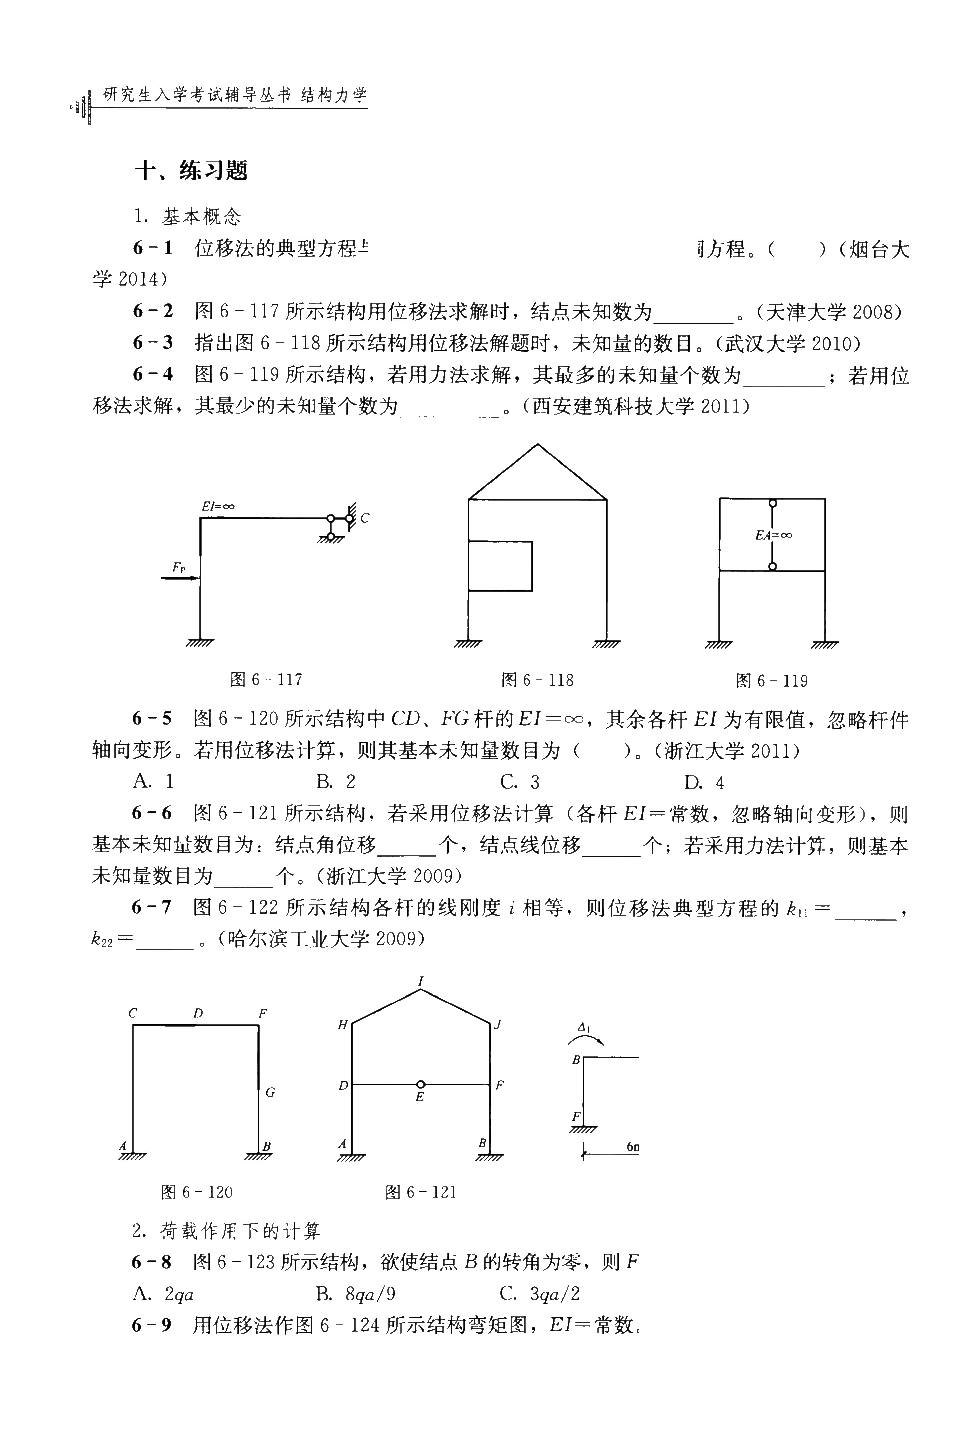
\includegraphics[width=0.92\textwidth]{figures/src15_p001.jpg}
\caption{结构力学基础与技巧班第12次作业及答案（位移法） 第 1 页清理图形页}
\end{figure}
\subsection*{第 2 页转写}
6-10

用位移法作图6－125所示结构的弯矩图。（福州大学2011)

2E

EI

EI

EI

图6-124

图6-123

图6-125

6 - 11

用位移法计算图6-126所示结构，作其弯矩图。各受弯杆件EI=常数。（湖南

大学2011)

6-12

用位移法求图6-127所示无侧移刚架的杆端弯矩，并绘制弯矩图。设已知各杆

件的相对线刚度：横梁为1，竖柱为1.5。（中国地震局工程力学研究所2011）

60kN

21kN/m

150kN-m

Fp=ql

2ml2m

1/2

8m

图6-126

图6-127

6-13

用位移法求解图6-128所示结构，作M图。EI为常数。（青岛理工大学2010）

6-14

用位移法计算图6－129所示结构并作其弯矩图。（西安建筑科技大学2008）

1.5EI

34kN/m

3kN/m

16kNm

EI

3EI

EI

1.5E1

4m

5m

8m

图6-128

图6-129

3.刚度无穷大杆件的计算

6-15图6-130所示结构中截面A弯矩Ms=

侧受拉。（哈尔

业大学2011)
\begin{figure}[H]\centering
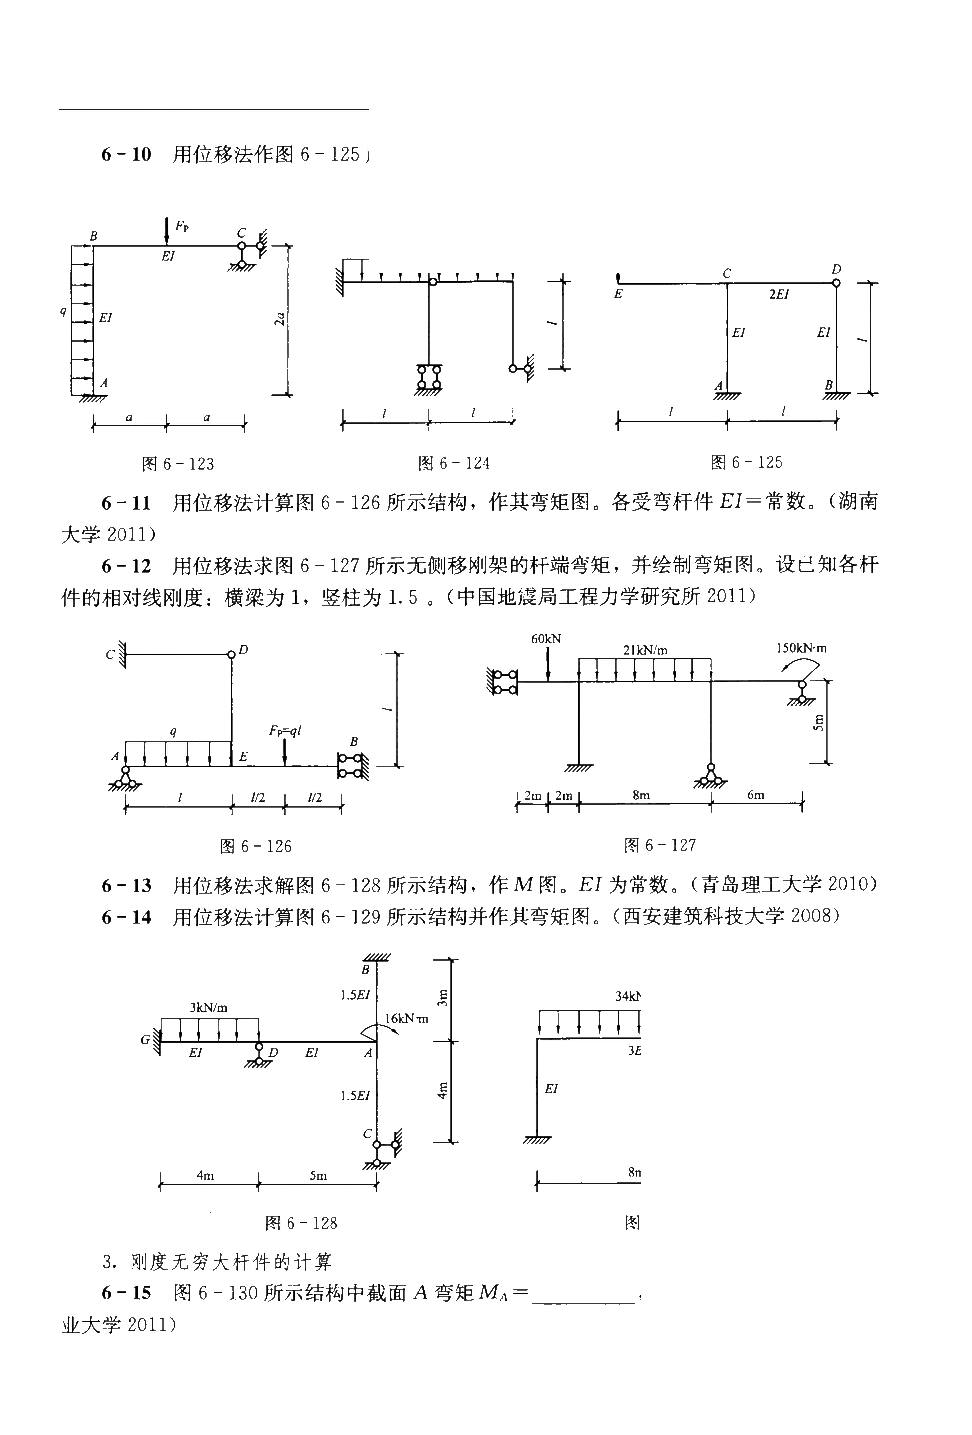
\includegraphics[width=0.92\textwidth]{figures/src15_p002.jpg}
\caption{结构力学基础与技巧班第12次作业及答案（位移法） 第 2 页清理图形页}
\end{figure}
\subsection*{第 3 页转写}
研究生入学考试辅导丛书结构力学（第二版）

6-16试用位移法计算图6-131所示刚架（EI=常数），并绘制其弯矩图。（湖南大学

2008)

12kN/m

EI

EI

El,=00

EI,

El,=

EI

EI

EI

EI

EI

4m

4m

图6-130

图6-131

6-17

作图6-132所示结构的M图、F。图及F\textasciitilde{}图。（中国矿业大学2009）

6-18用位移法作图6-133所示结构的M图。设横梁EI为无限大，各柱相对线刚度

如图中所示。（华南理工大学2010）

EI

E=080

EI

EI

21

10m

图6-132

图6-133

4.对称性的利用

6-19

用位移法求图6－134所示结构的弯矩图。EI=常数。（北京工业大学2013）

6-20

用位移法作图6-135所示结构弯矩图。EI=常数。（苏州科技学院2007、华南

理工大学2006）

图6-134

图6-135

308
\begin{figure}[H]\centering
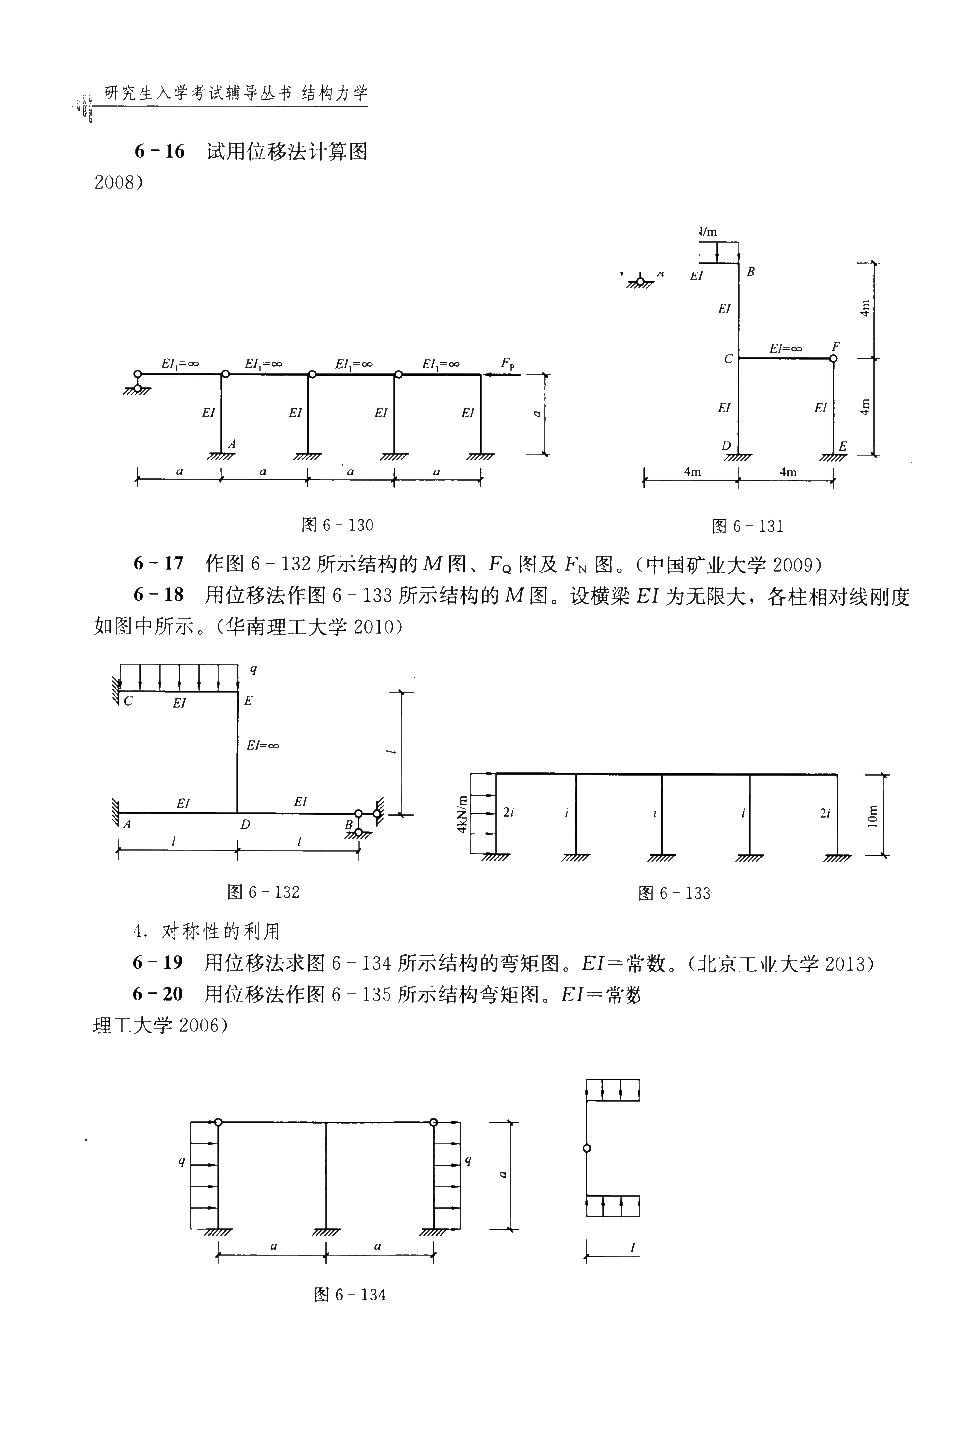
\includegraphics[width=0.92\textwidth]{figures/src15_p003.jpg}
\caption{结构力学基础与技巧班第12次作业及答案（位移法） 第 3 页清理图形页}
\end{figure}
\subsection*{第 4 页转写}
6- 21

作图6-136所示结构的M图，各杆EI=常数。（西南交通大学2010)

6-22

用位移法作图6-137所示结构M图。各杆EI=常数。（山东建筑大学2012）

4kN/m

21

3m

3m

1/2

1/2

图6-136

图6-137

6-23 用位移法作图6-138所示结构M图。各杆EI=常数。（山东建筑大学2009）

6-24

用位移法作图6-139所示结构M图。已知各杆EI=常数。（广西大学2010年）

40kN

1/2

1/2

1/2

1/2

4m

1/2

4m

图6-138

图6-139

6-25用合适的方法计算图6-140所示对称结构，并作出M图。EI=常数。（中国矿

业大学2011)

6-26

根据对称性用位移法求解图6-141所示结构，作M图。EI为常数。（青岛理工

大学2012)

12kN

3kN/m

EI

10kN/m

10kN/m

EI

6m

4m

4m

2m/2m

4m

4m

图6-140

图6-141

6-27

用位移法作图6-142所示结构的M图。EI=常数。（烟台大学2013）

309！
\begin{figure}[H]\centering
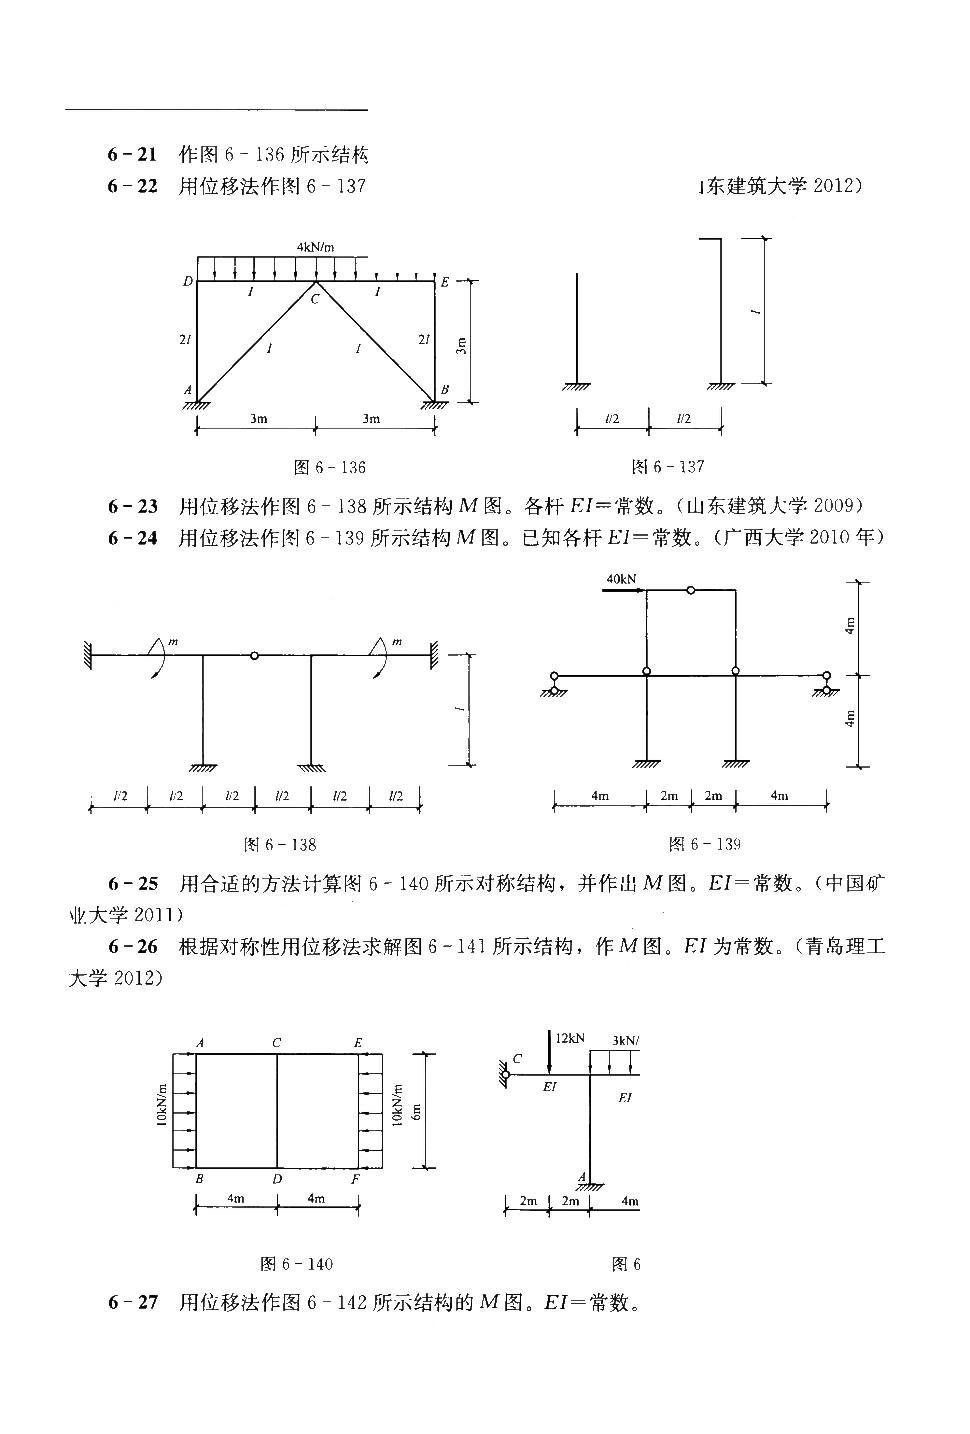
\includegraphics[width=0.92\textwidth]{figures/src15_p004.jpg}
\caption{结构力学基础与技巧班第12次作业及答案（位移法） 第 4 页清理图形页}
\end{figure}
\subsection*{第 5 页转写}
研究生入学考试辅导丛书结构力学（第二版）

5.不需计算绘制弯矩图的形状

6-28画出图6-143（a）、（b）所示结构弯矩图的轮廓，杆件抗弯刚度EI=常数。

（北京交通大学2010）

FP

+I'C

Fp

(a)

(b)

图6-142

图6-143

6-29定性地画出图6-144所示结构在图示荷载作用下弯矩图的大致形状。（武汉理

工大学2010)

6.弹性支承超静定结构的计算

6-30用位移法计算图6-145所示结构并作M图，中间支座为弹性支座，其刚度系

数k=5EI/3，EI=常数。（合肥工业大学2009）

Fp

1/2

1/2

图6-144

图6-145

7.支座位移和温度改变时的计算

6-31用位移法求解图6-146所示结构的M图（须写出计算过程）。（已知：EI=4.8X

10*kN m ）（东南大学2007）

6-32图6-147所示刚架，B支座产生竖向位移$\triangle$时，试用位移法作弯矩图。（天津

大学2008)

21

0.02m

6m

6m

图6-146

图6-147

8.用位移法求超静定结构的位移

6-33用位移法求解图6-148所示结构未知结点位移。（东南大学2013）

310
\begin{figure}[H]\centering
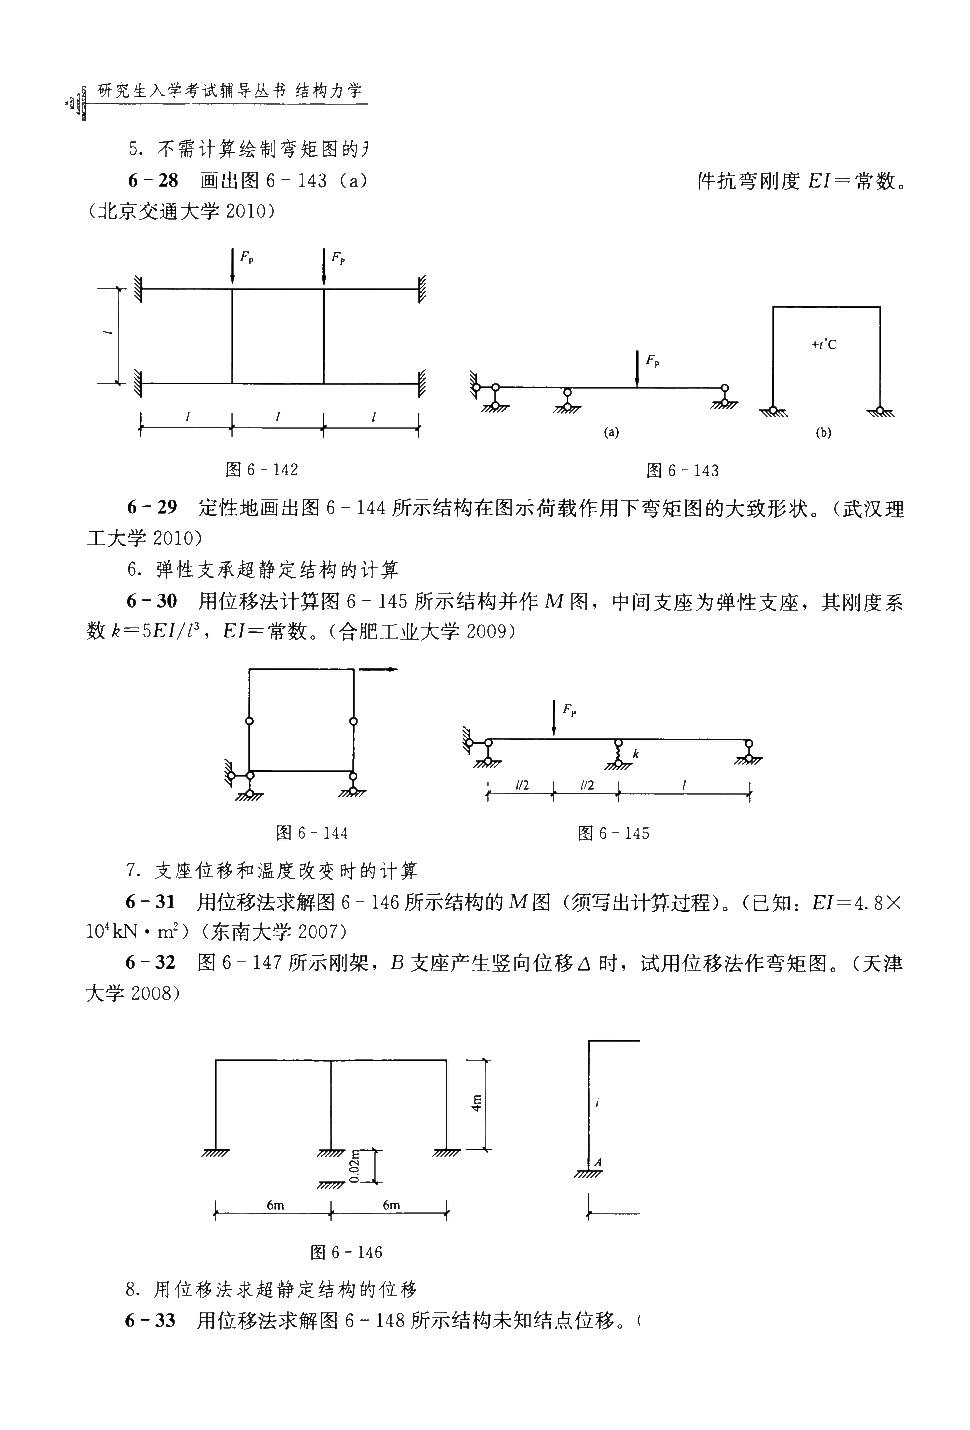
\includegraphics[width=0.92\textwidth]{figures/src15_p005.jpg}
\caption{结构力学基础与技巧班第12次作业及答案（位移法） 第 5 页清理图形页}
\end{figure}
\subsection*{第 6 页转写}
6-34图6-149所示结构各杆抗弯刚度EI为常数，BC杆受到均布荷载作用，同时D

支座下沉$\triangle$。试求B结点转角，并画出变形图的大致形状。（武汉理工大学2010）

EI

El=

2ql

图6-148

图6-149
\begin{figure}[H]\centering
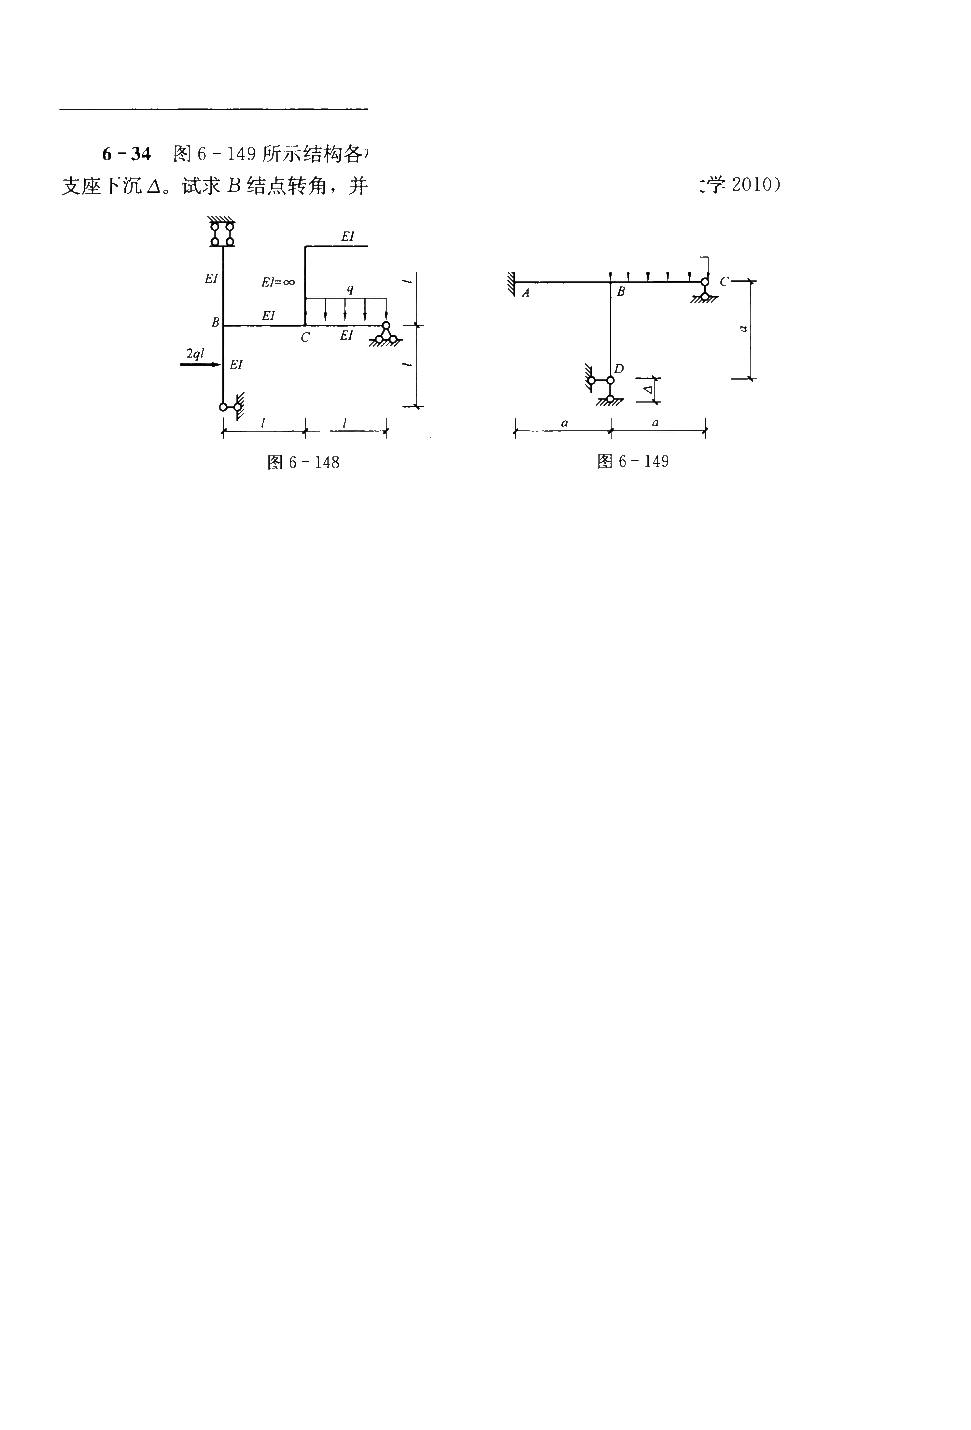
\includegraphics[width=0.92\textwidth]{figures/src15_p006.jpg}
\caption{结构力学基础与技巧班第12次作业及答案（位移法） 第 6 页清理图形页}
\end{figure}
\subsection*{第 7 页转写}
6-1、

6-2、17

6-3、119

6-P

线作袋：4
\begin{figure}[H]\centering
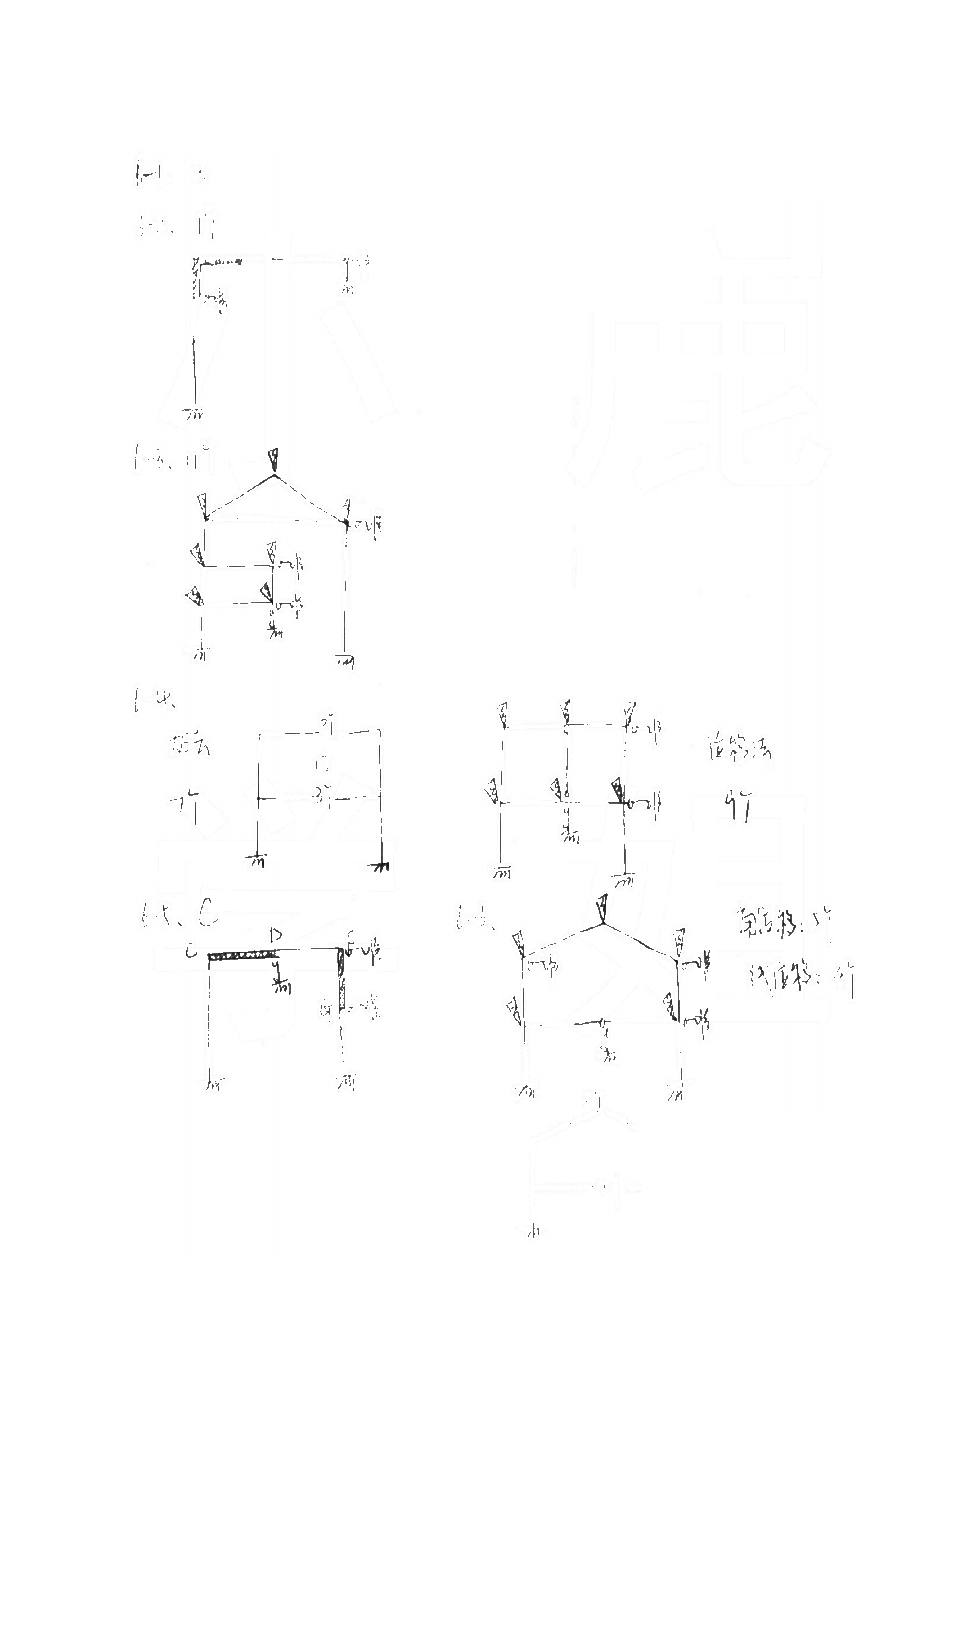
\includegraphics[width=0.92\textwidth]{figures/src15_p007.jpg}
\caption{结构力学基础与技巧班第12次作业及答案（位移法） 第 7 页清理图形页}
\end{figure}
\subsection*{第 8 页转写}
6-8

72

MA
\begin{figure}[H]\centering
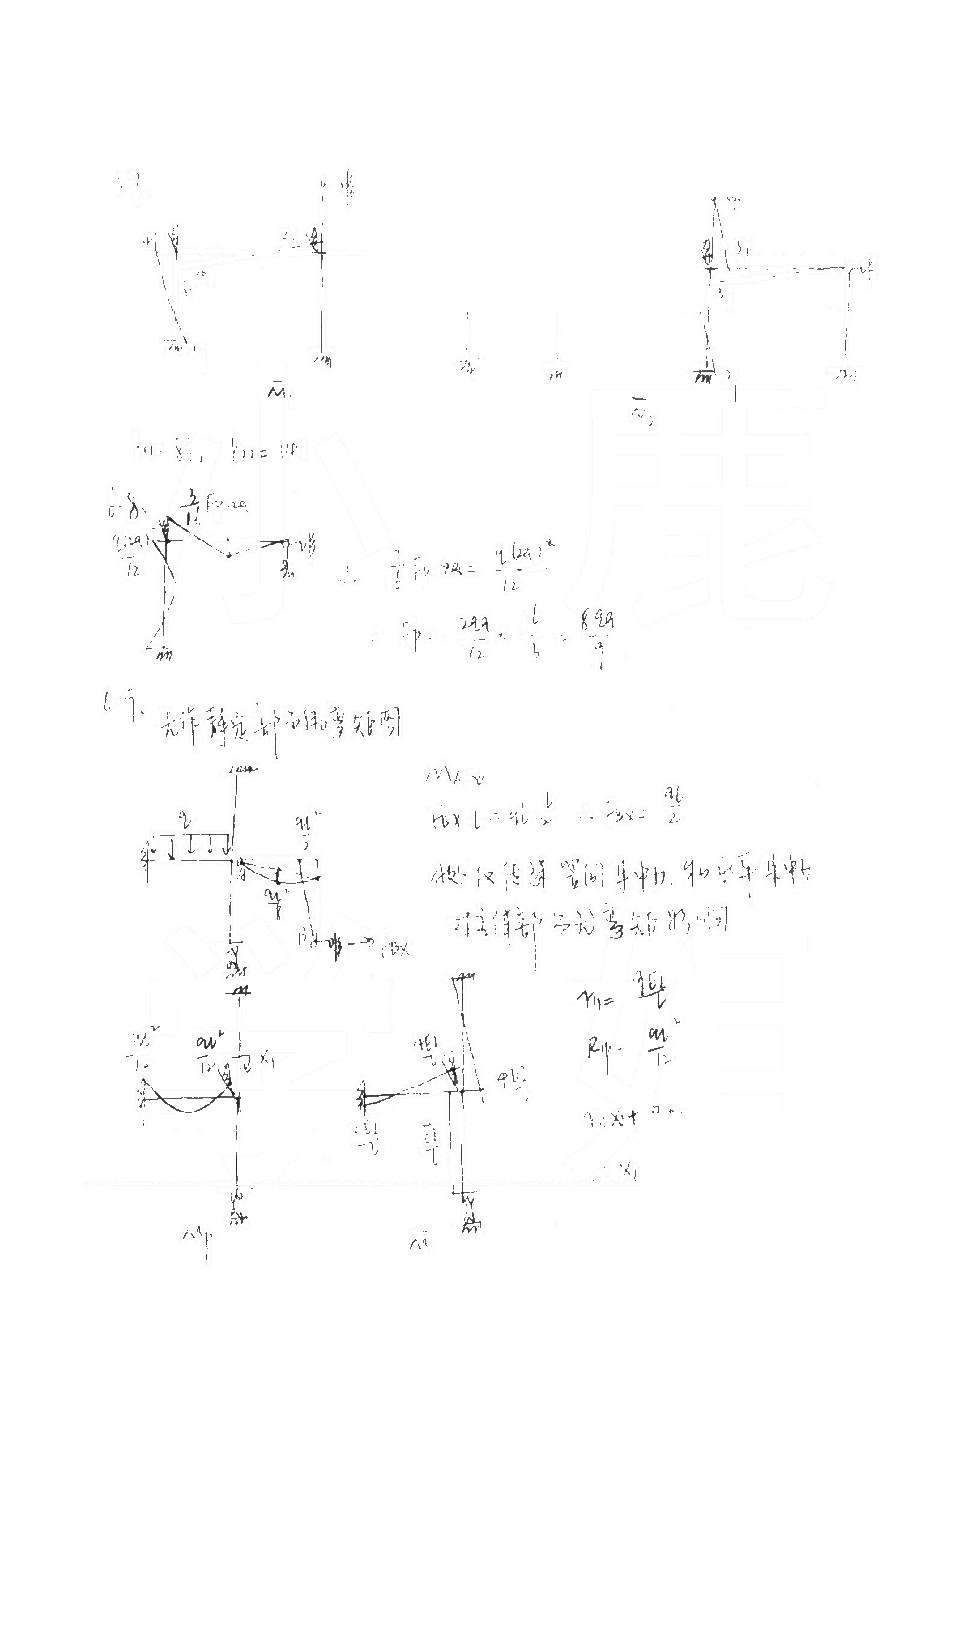
\includegraphics[width=0.92\textwidth]{figures/src15_p008.jpg}
\caption{结构力学基础与技巧班第12次作业及答案（位移法） 第 8 页清理图形页}
\end{figure}
\subsection*{第 9 页转写}
T08

6 0.

M2

73

19
\begin{figure}[H]\centering
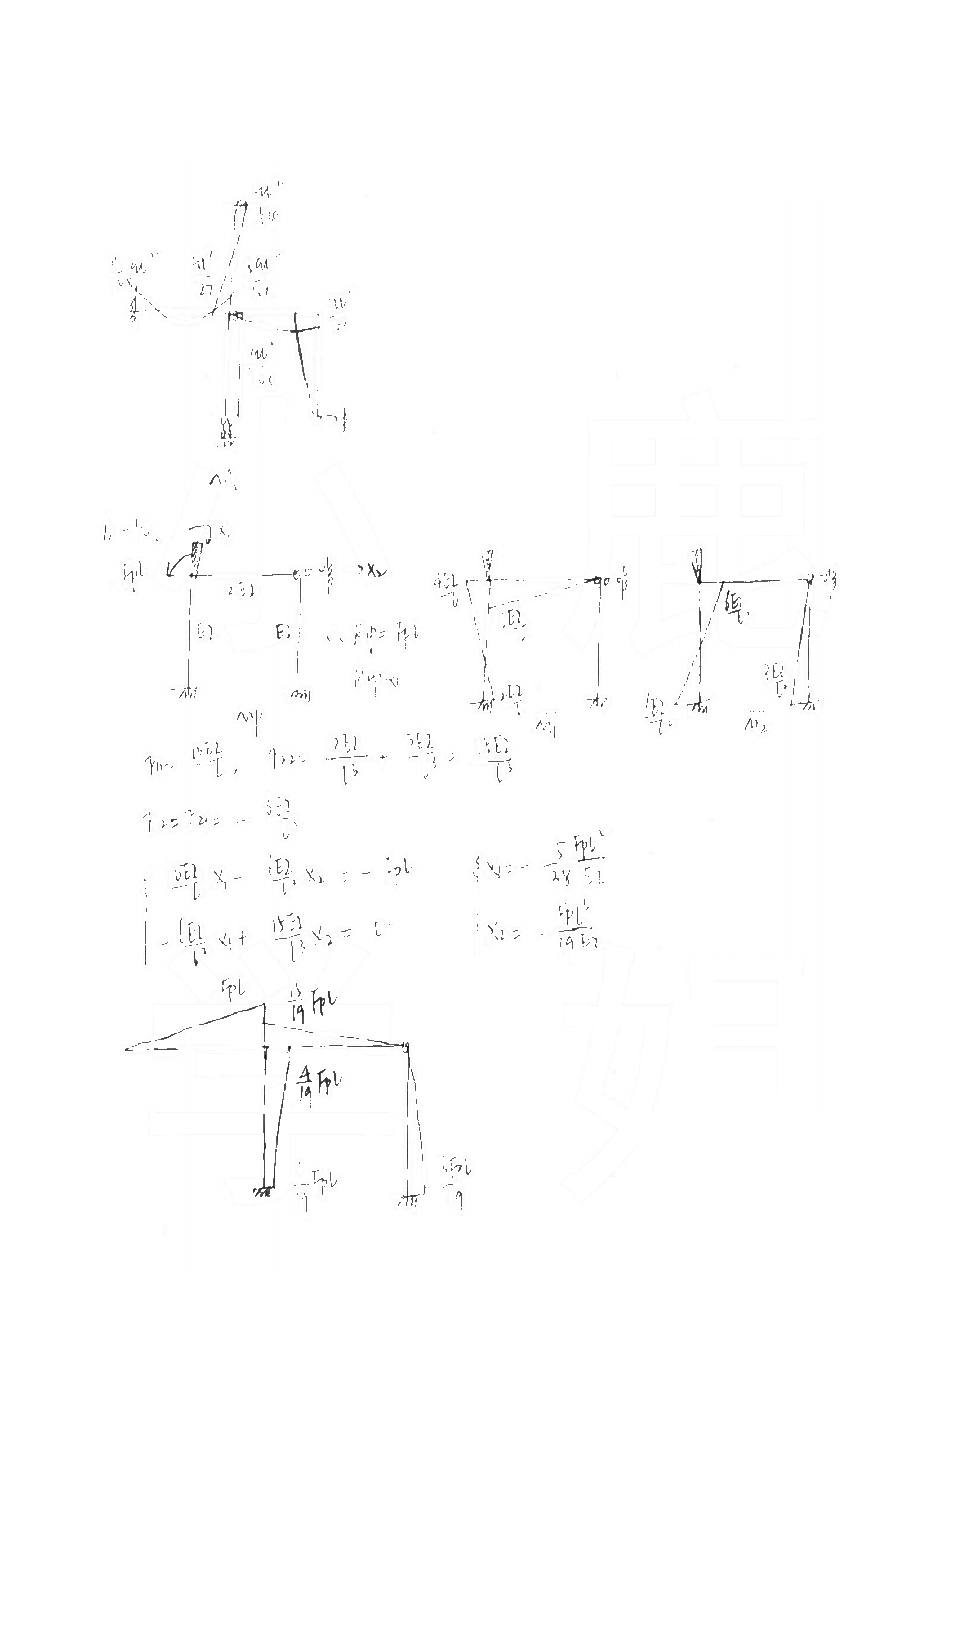
\includegraphics[width=0.92\textwidth]{figures/src15_p009.jpg}
\caption{结构力学基础与技巧班第12次作业及答案（位移法） 第 9 页清理图形页}
\end{figure}
\subsection*{第 10 页转写}
6-1.

612.

l号$\times$b$\times$40vm

=1237m
\begin{figure}[H]\centering
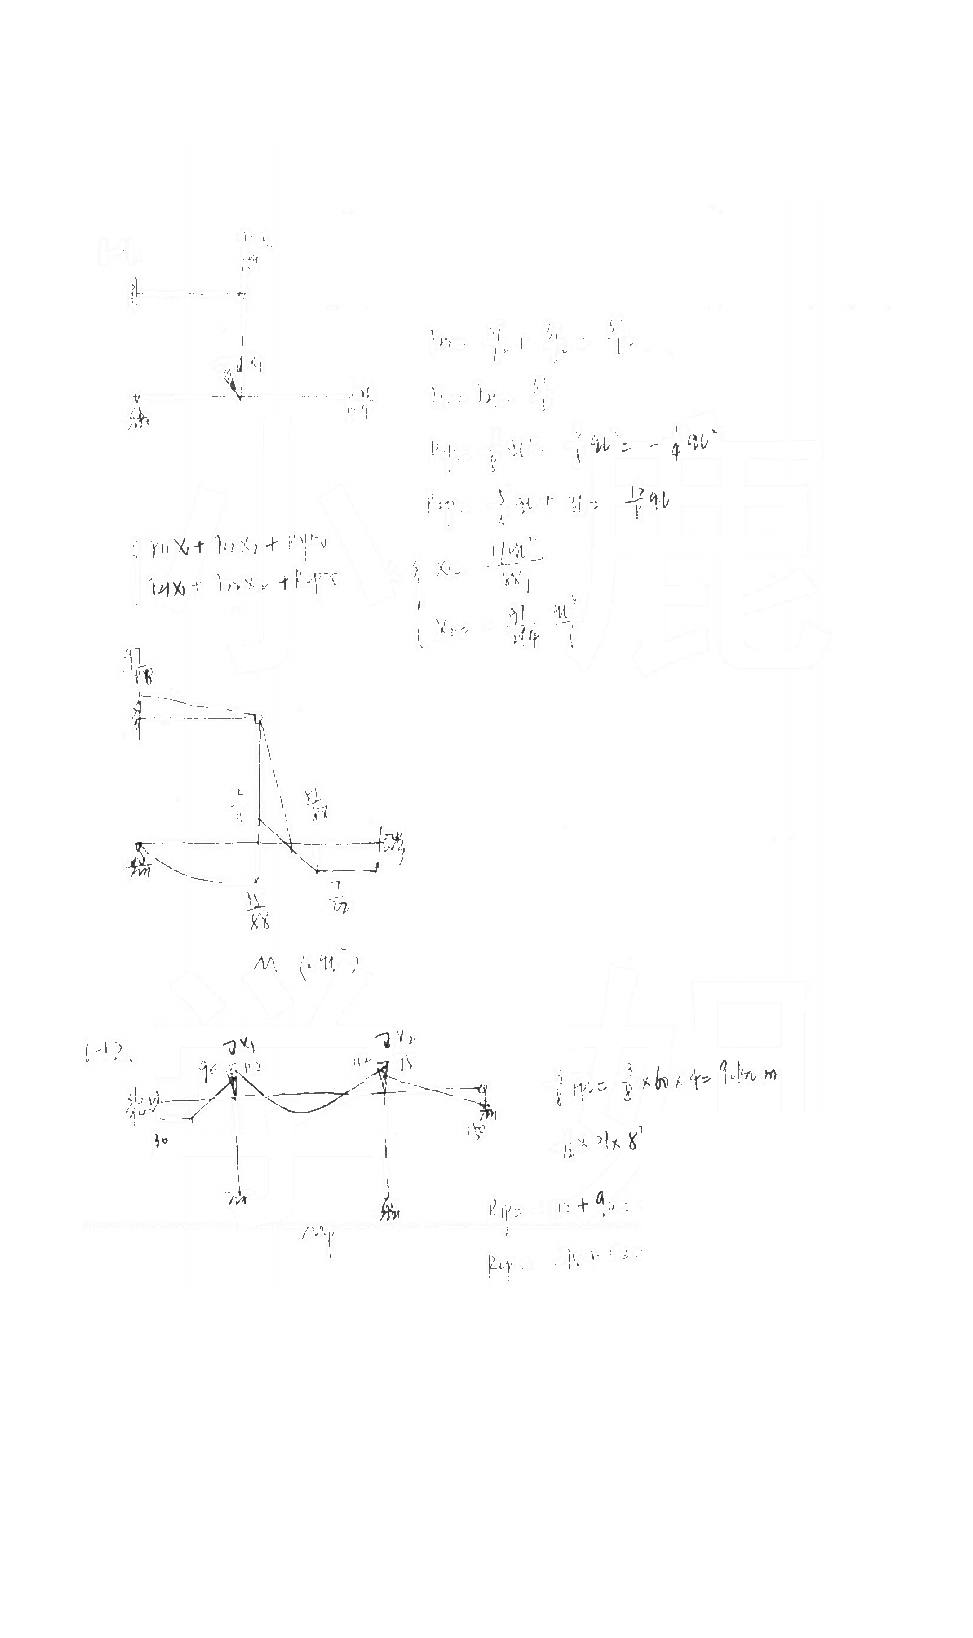
\includegraphics[width=0.92\textwidth]{figures/src15_p010.jpg}
\caption{结构力学基础与技巧班第12次作业及答案（位移法） 第 10 页清理图形页}
\end{figure}
\subsection*{第 11 页转写}
X=2.67

X-3.68

108.68

9247

ha98 29z01

2733 602

613

Pps

19

432
\begin{figure}[H]\centering
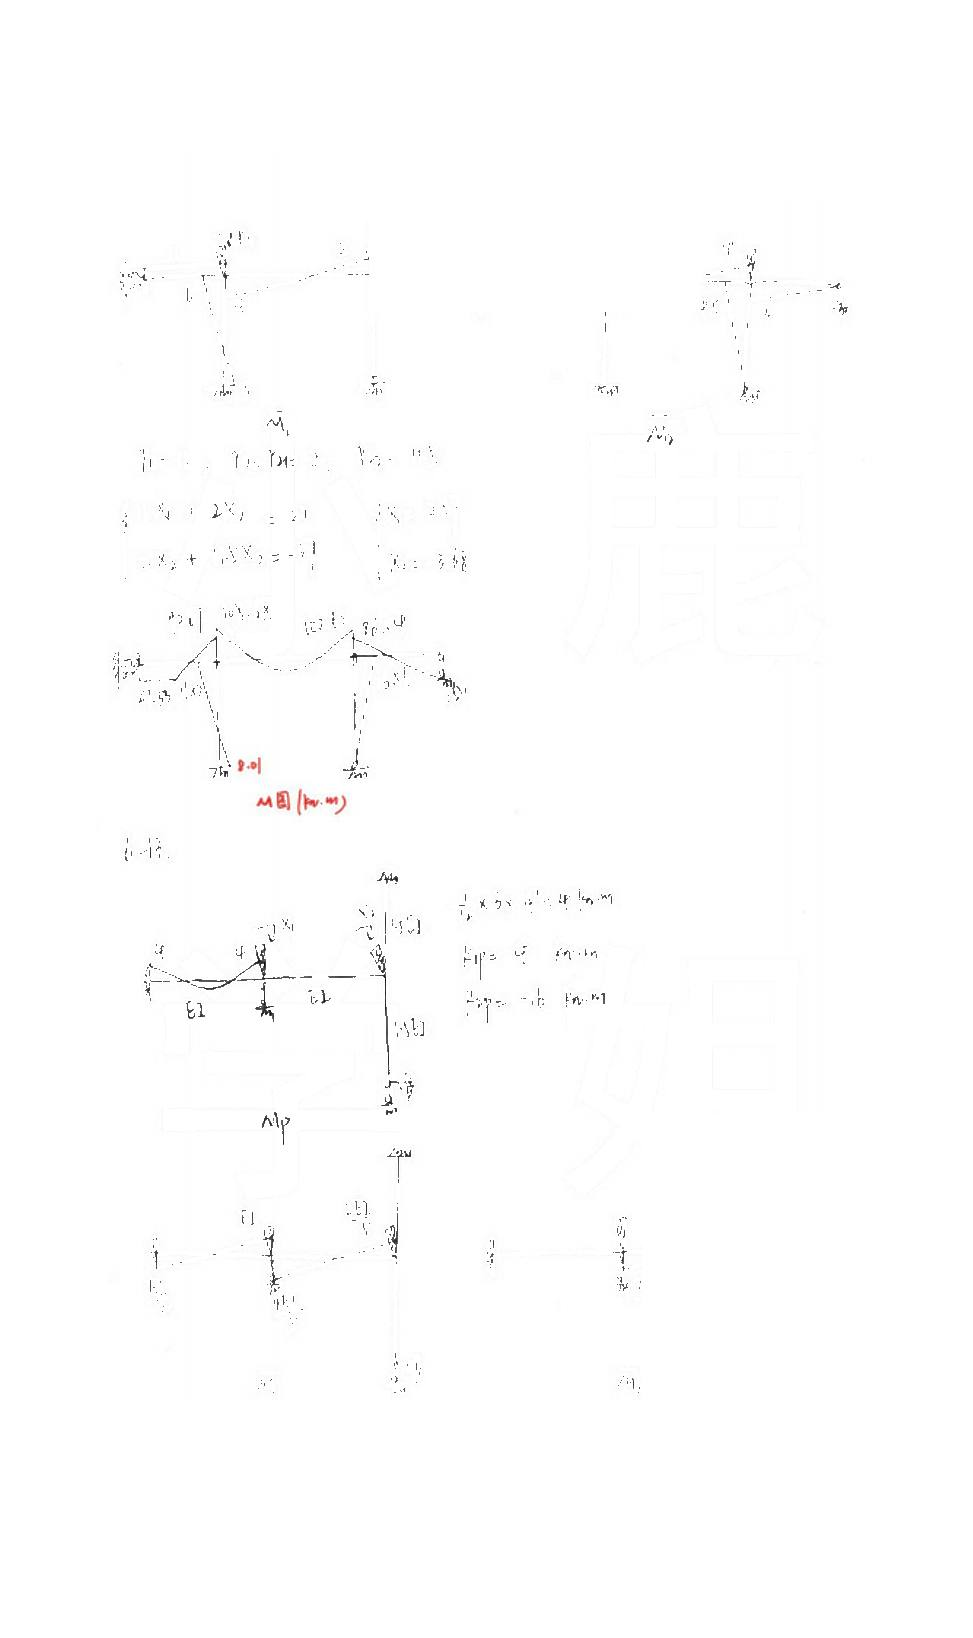
\includegraphics[width=0.92\textwidth]{figures/src15_p011.jpg}
\caption{结构力学基础与技巧班第12次作业及答案（位移法） 第 11 页清理图形页}
\end{figure}
\subsection*{第 12 页转写}
7852

Ins

78.5

08

6-4
\begin{figure}[H]\centering
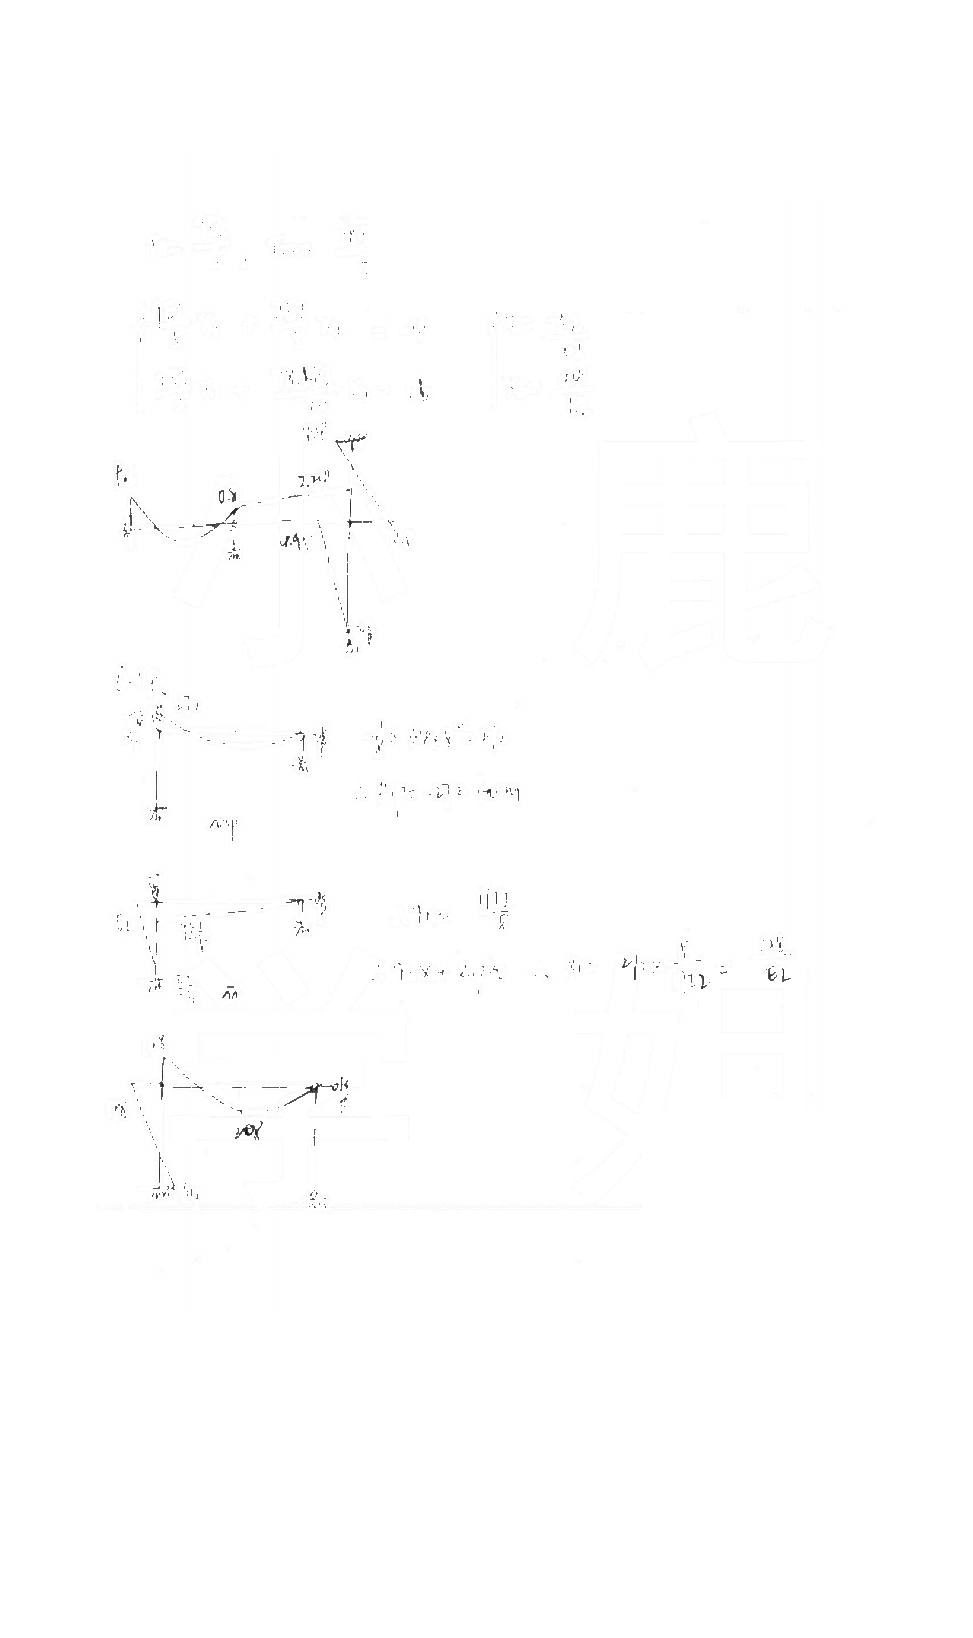
\includegraphics[width=0.92\textwidth]{figures/src15_p012.jpg}
\caption{结构力学基础与技巧班第12次作业及答案（位移法） 第 12 页清理图形页}
\end{figure}
\subsection*{第 13 页转写}
615、

72
\begin{figure}[H]\centering
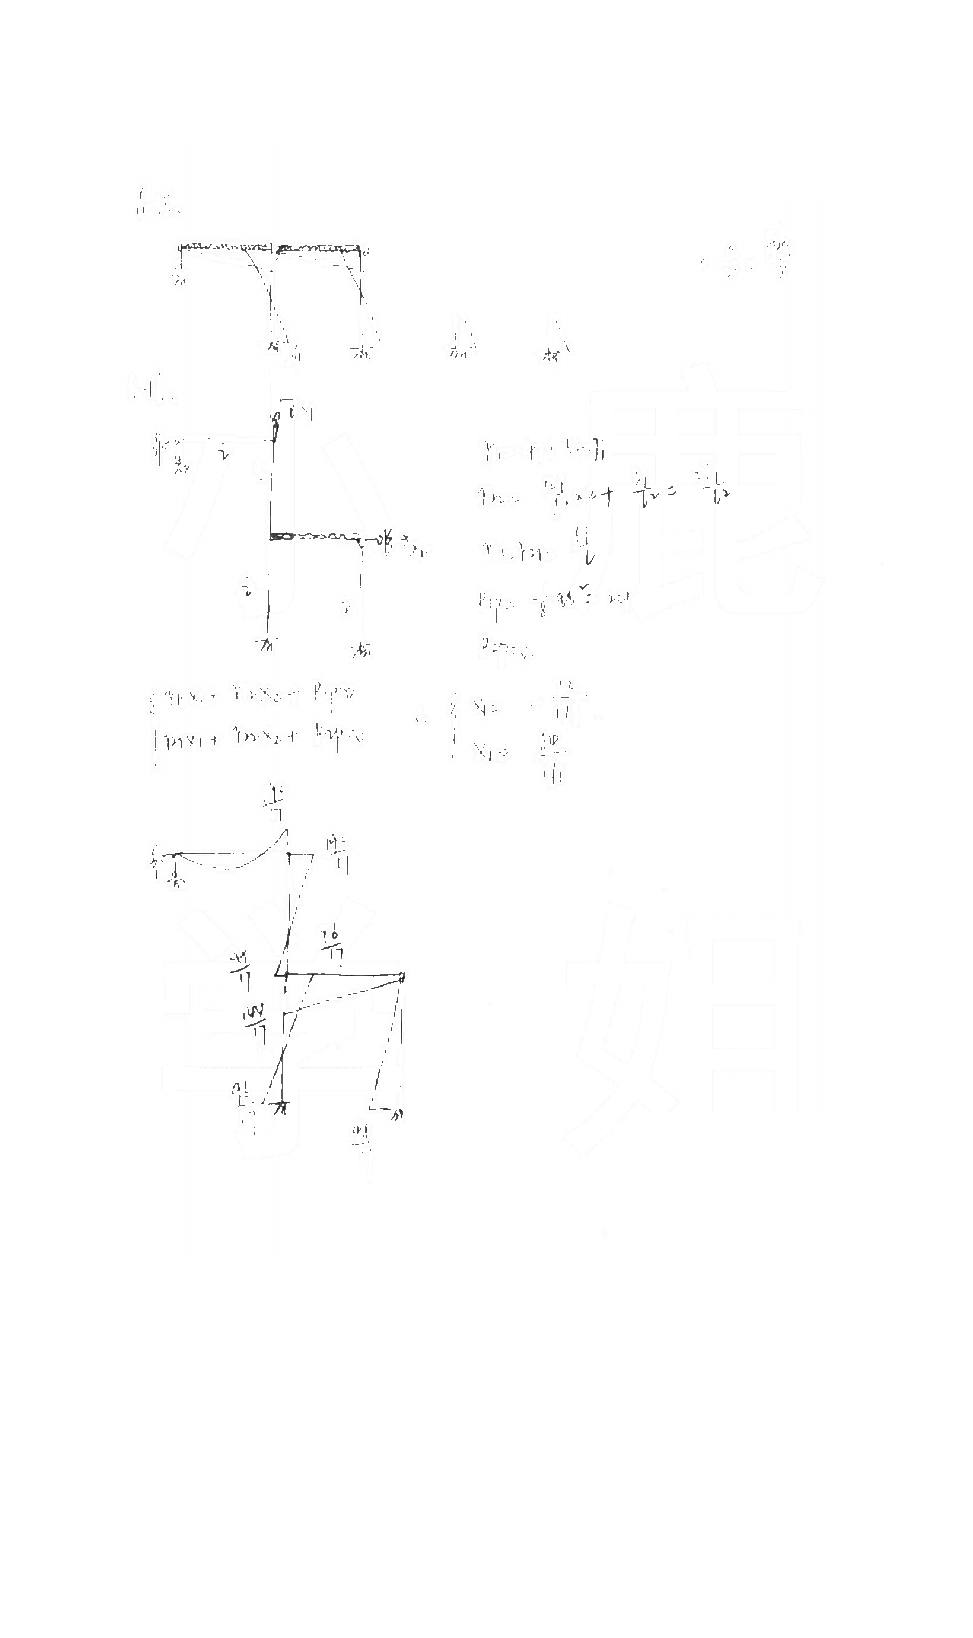
\includegraphics[width=0.92\textwidth]{figures/src15_p013.jpg}
\caption{结构力学基础与技巧班第12次作业及答案（位移法） 第 13 页清理图形页}
\end{figure}
\subsection*{第 14 页转写}
X=

13g/18

9/12

Spl/18

5g/18

18

gh12

2gl9

9124

g124

g/18

M图

Fom

FM

618

10
\begin{figure}[H]\centering
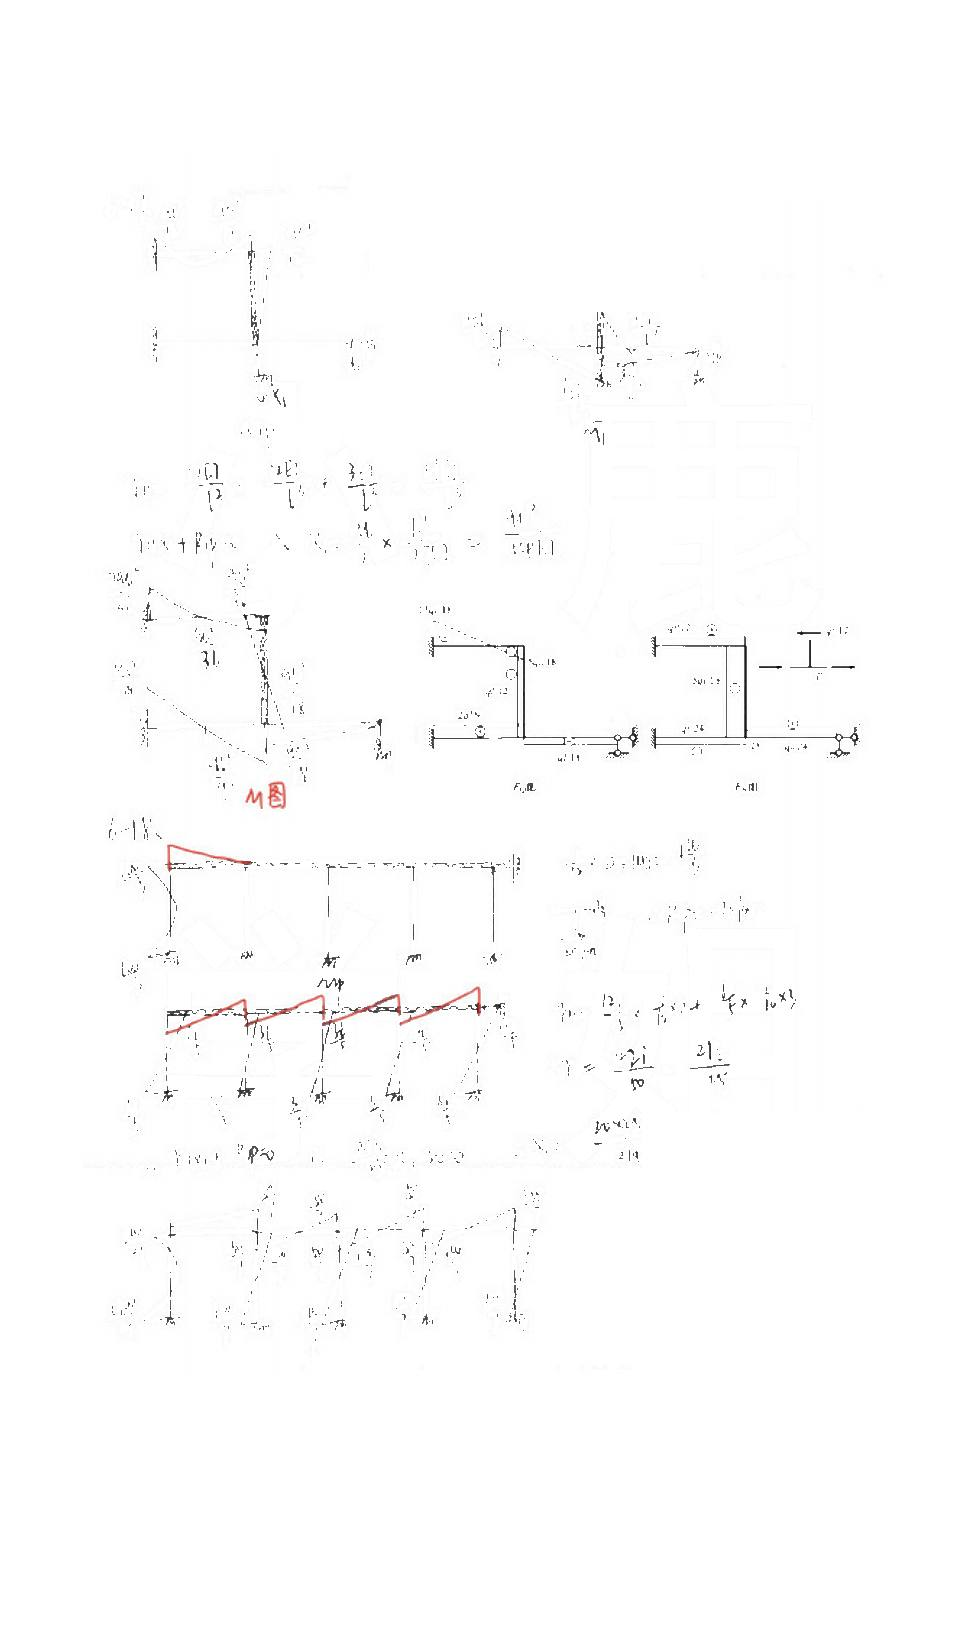
\includegraphics[width=0.92\textwidth]{figures/src15_p014.jpg}
\caption{结构力学基础与技巧班第12次作业及答案（位移法） 第 14 页清理图形页}
\end{figure}
\subsection*{第 15 页转写}
\emph{本页原始资料主要为结构图、手写推导或扫描图形；已在下方清理图形页保留。}
\begin{figure}[H]\centering
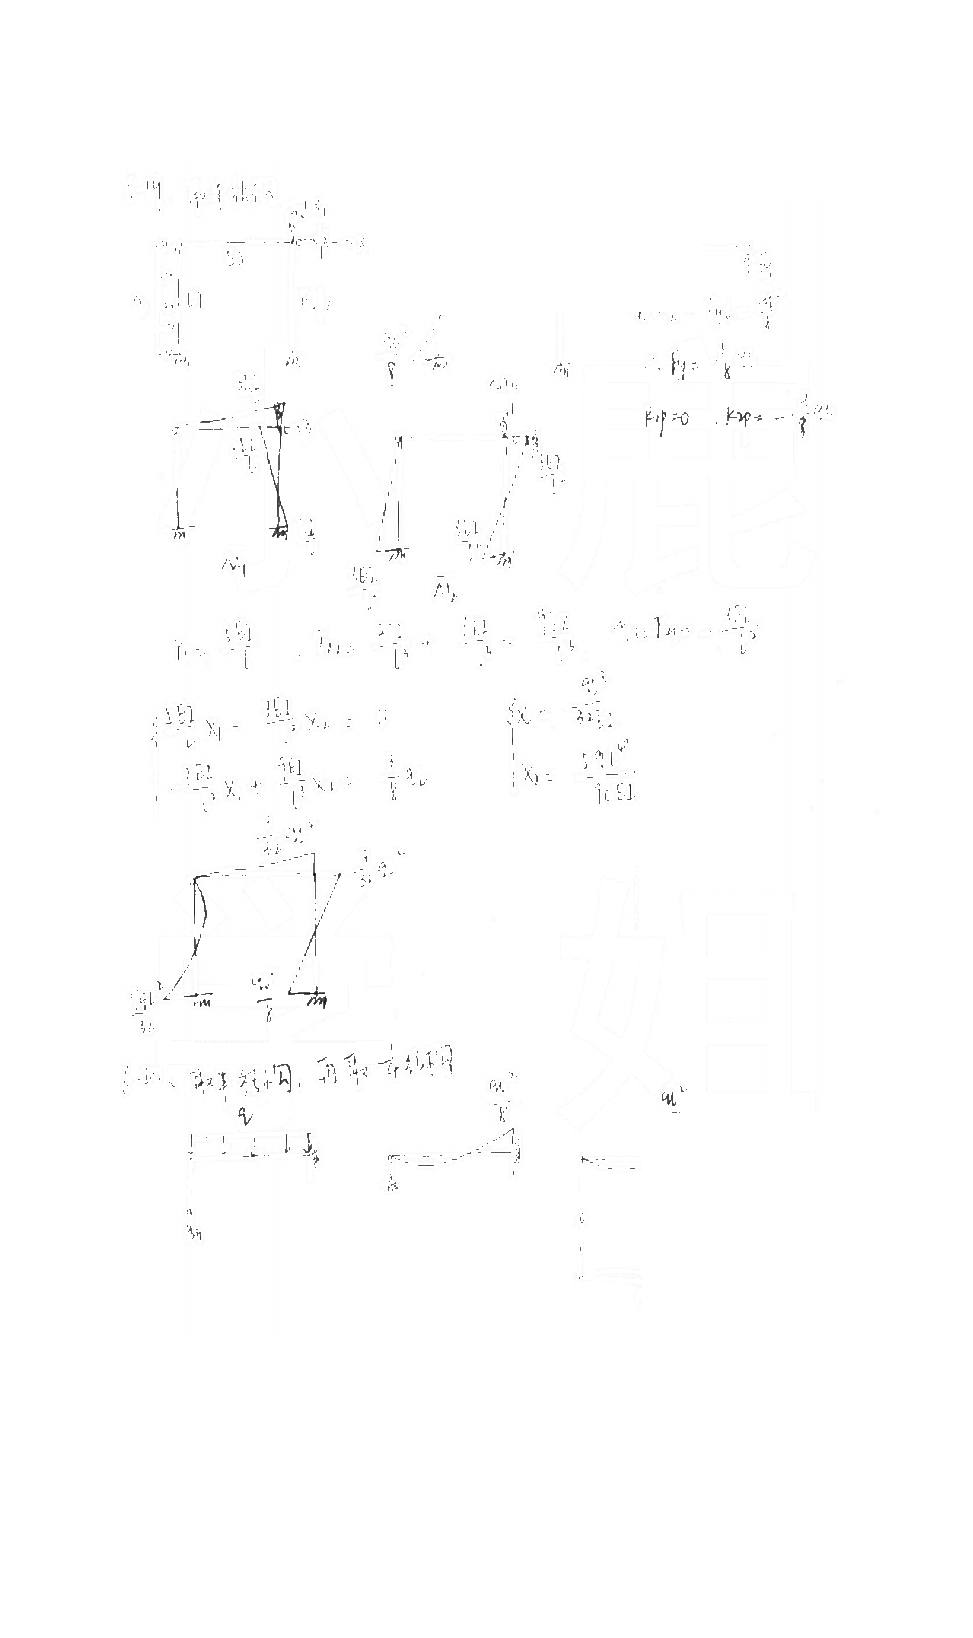
\includegraphics[width=0.92\textwidth]{figures/src15_p015.jpg}
\caption{结构力学基础与技巧班第12次作业及答案（位移法） 第 15 页清理图形页}
\end{figure}
\subsection*{第 16 页转写}
-9
\begin{figure}[H]\centering
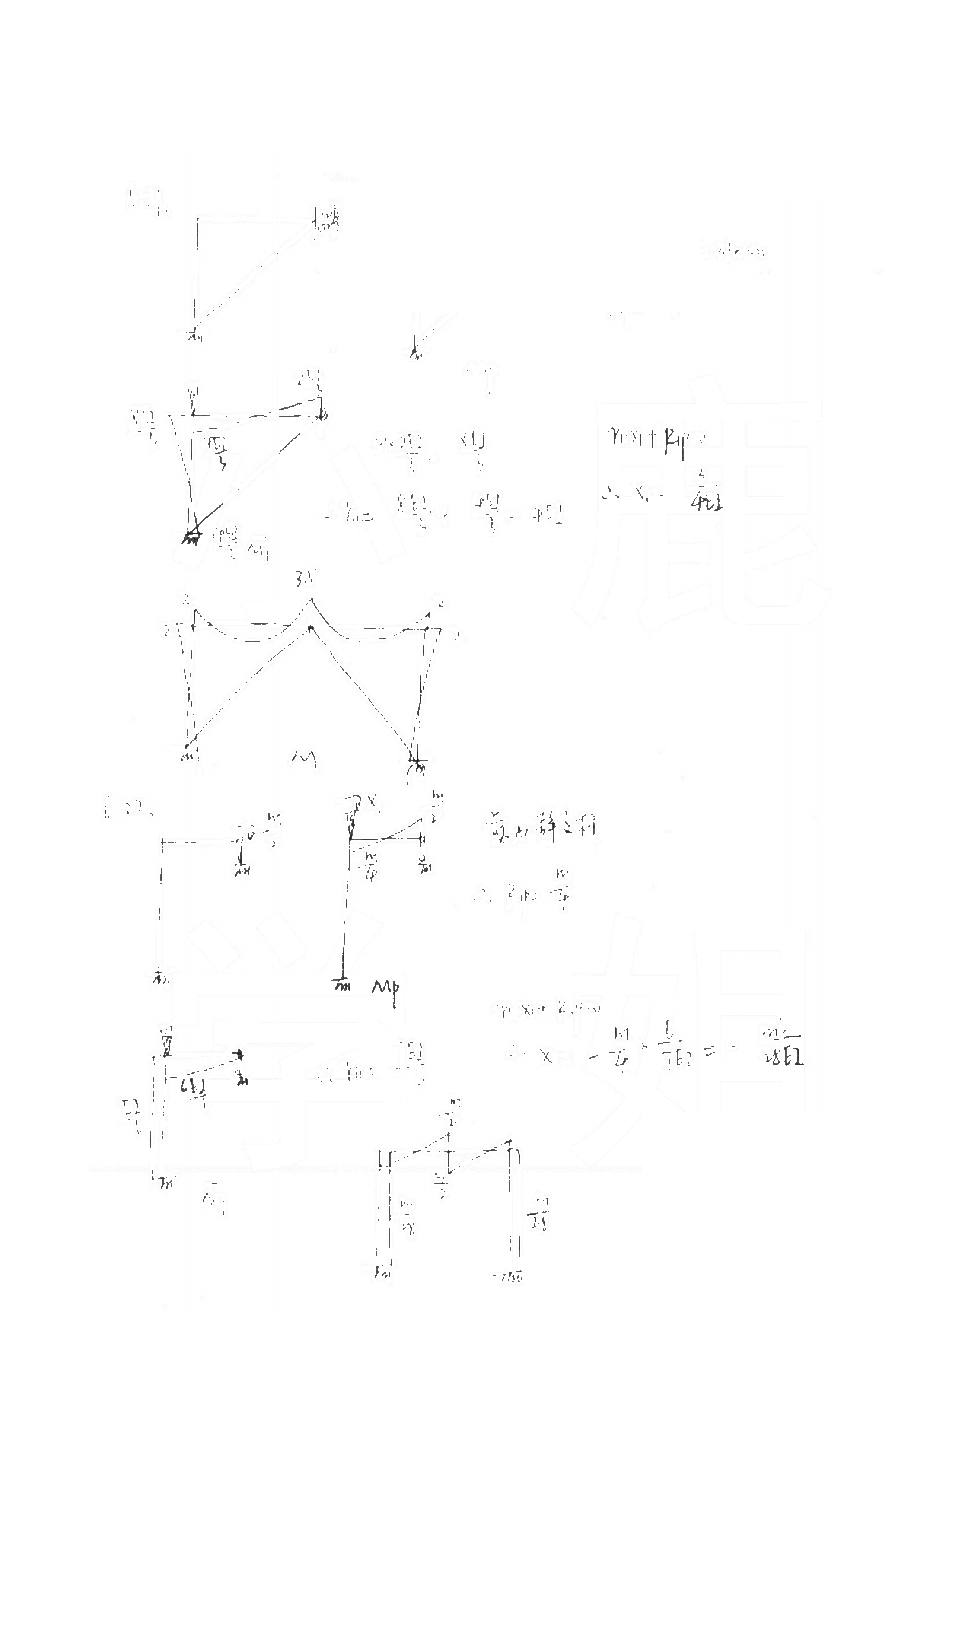
\includegraphics[width=0.92\textwidth]{figures/src15_p016.jpg}
\caption{结构力学基础与技巧班第12次作业及答案（位移法） 第 16 页清理图形页}
\end{figure}
\subsection*{第 17 页转写}
Yh=

MP

6-24

40

36

12

M(pwn)
\begin{figure}[H]\centering
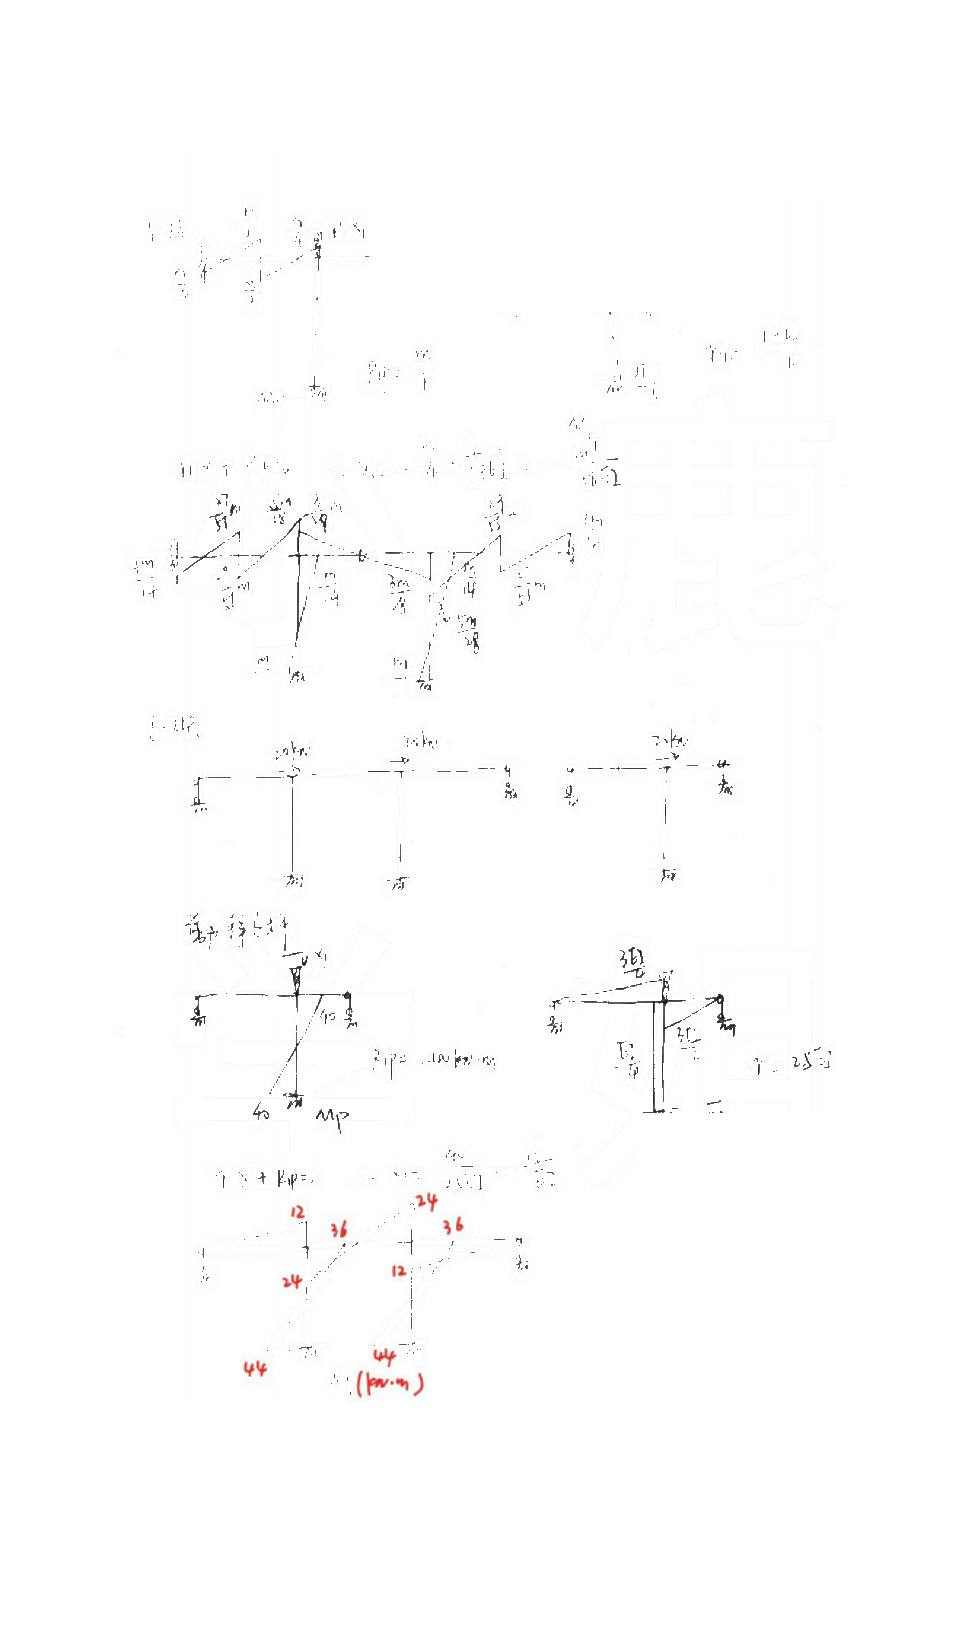
\includegraphics[width=0.92\textwidth]{figures/src15_p017.jpg}
\caption{结构力学基础与技巧班第12次作业及答案（位移法） 第 17 页清理图形页}
\end{figure}
\subsection*{第 18 页转写}
6-25、

解：依次取正对称半结构和四分之一结构如图所示，位移法基本体系见图（a），位移法方

程为11

1

1

0

P

r X

R

+

=

。画出

1

M 图和M P 图如图（b）（c）所示，各系数和自由项为

11

4

3

EI

r =

，

1

30

P

R

=

将系数和自由项代入位移法方程

1

4

30

0

3

EI X +

=

，解方程得

1

45

2

X

EI

=  

。由对称性

M=11 + M叠加得原结构最后弯矩图，如图（d）所示。

6-26、

解：可将原结构荷载分解为正对称和反对称两种情况，正对称情况下取半结构，位移法基

本体系见图（a），位移法方程为11

1

1

0

P

r X

R

+

=

。画出

1

M 图和M P 图如图（b）（c）所

示，各系数和自由项为

11

23

12

EI

r =

，

1

1

2

P

R

=

将系数和自由项代入位移法方程

1

23

1

0

12

2

EI X +

=

，解方程得

1

6

23

X

EI

=  

。由对称性

M=11 + M叠加得正对称结构弯矩图，如图（d）所示。
\begin{figure}[H]\centering
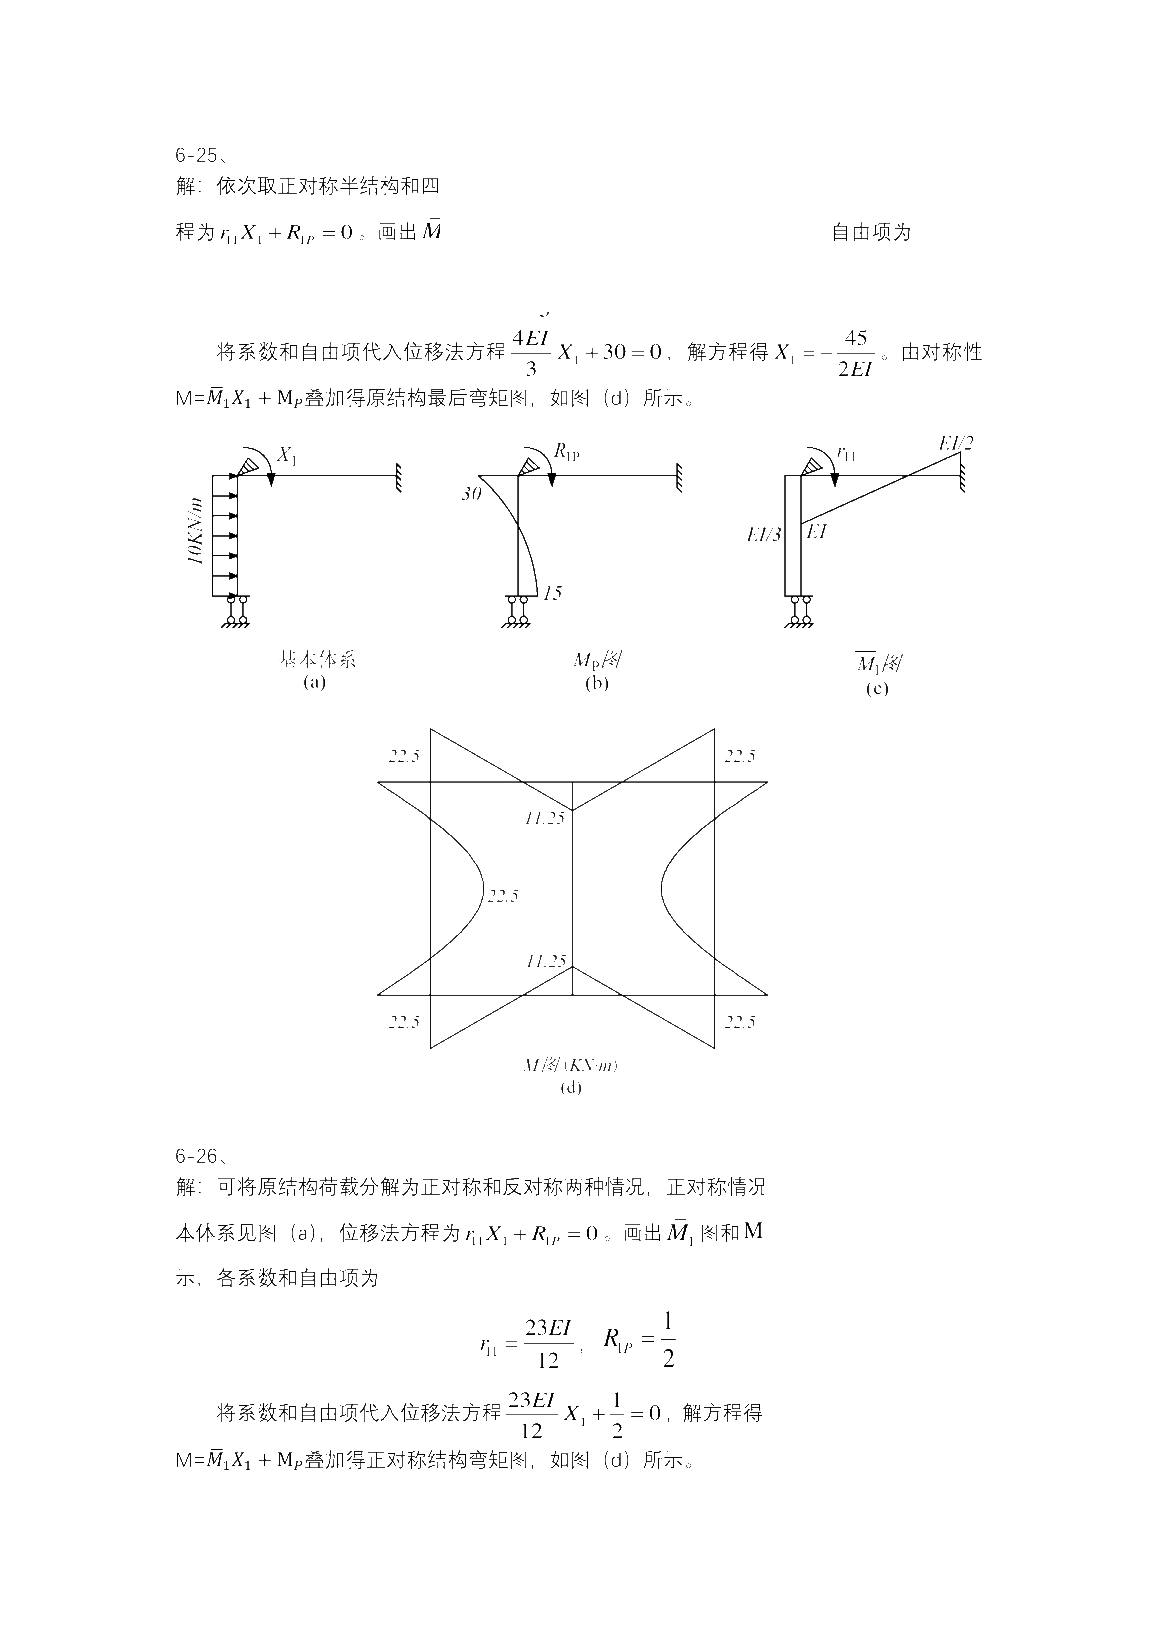
\includegraphics[width=0.92\textwidth]{figures/src15_p018.jpg}
\caption{结构力学基础与技巧班第12次作业及答案（位移法） 第 18 页清理图形页}
\end{figure}
\subsection*{第 19 页转写}
同理反对称情况下取半结构，位移法基本体系见图（e），取位移法方程为11

1

1

0

P

r X

R

+

=

。

画出

1

M 图和M P 图如图（f）（g）所示，各系数和自由项为

11

35

12

EI

r =

，

1

9

2

P

R

=

将系数和自由项代入位移法方程

1

35

9

0

12

2

EI X +

=

，解方程得

1

54

35

X

EI

=  

。由对称性

M=11 + M叠加得正对称结构弯矩图，如图（h）所示。综合以上计算，叠加正对称和反

对称情况下弯矩图可得原结构弯矩图如图（i）所示。
\begin{figure}[H]\centering
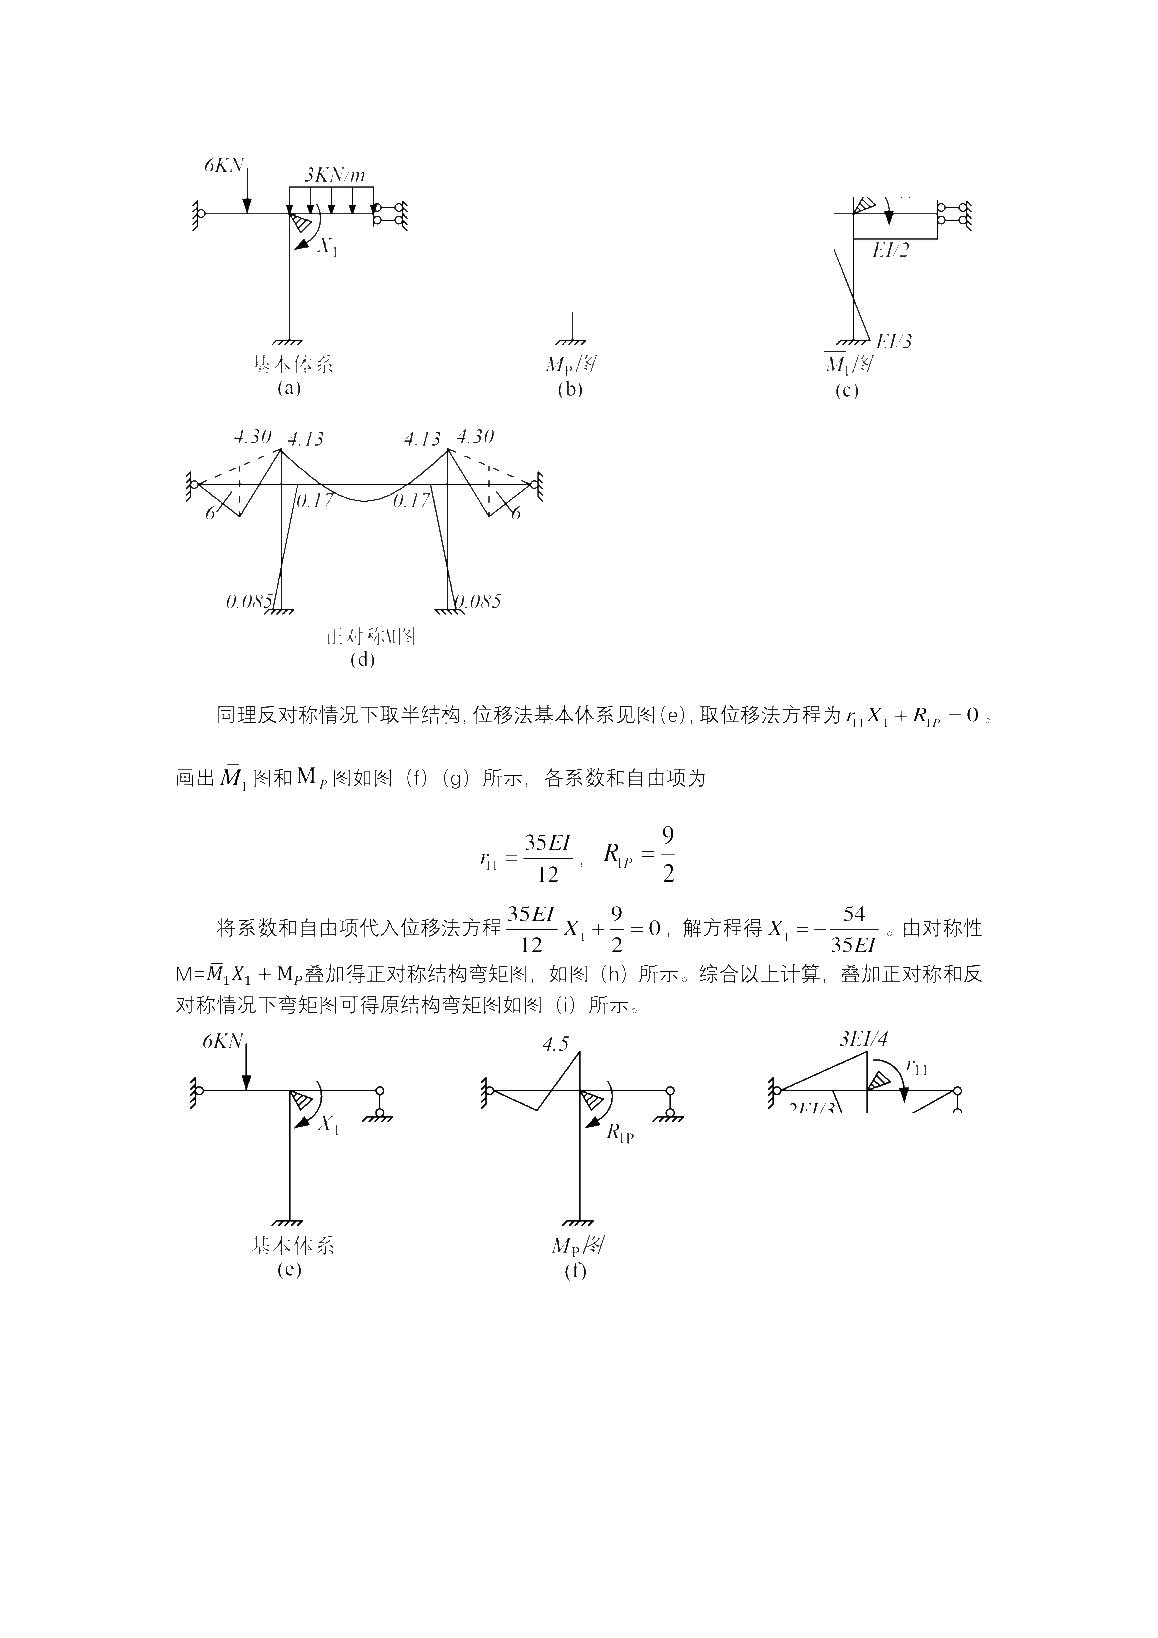
\includegraphics[width=0.92\textwidth]{figures/src15_p019.jpg}
\caption{结构力学基础与技巧班第12次作业及答案（位移法） 第 19 页清理图形页}
\end{figure}
\subsection*{第 20 页转写}
7.64,6.44

3.34

2.31

12

1.82.

0.96

1.03

0.86

2.31

3.34

0.515

0.515

0.6

0.43

反对称M图

M图(KN-m)

(h)

()
\begin{figure}[H]\centering
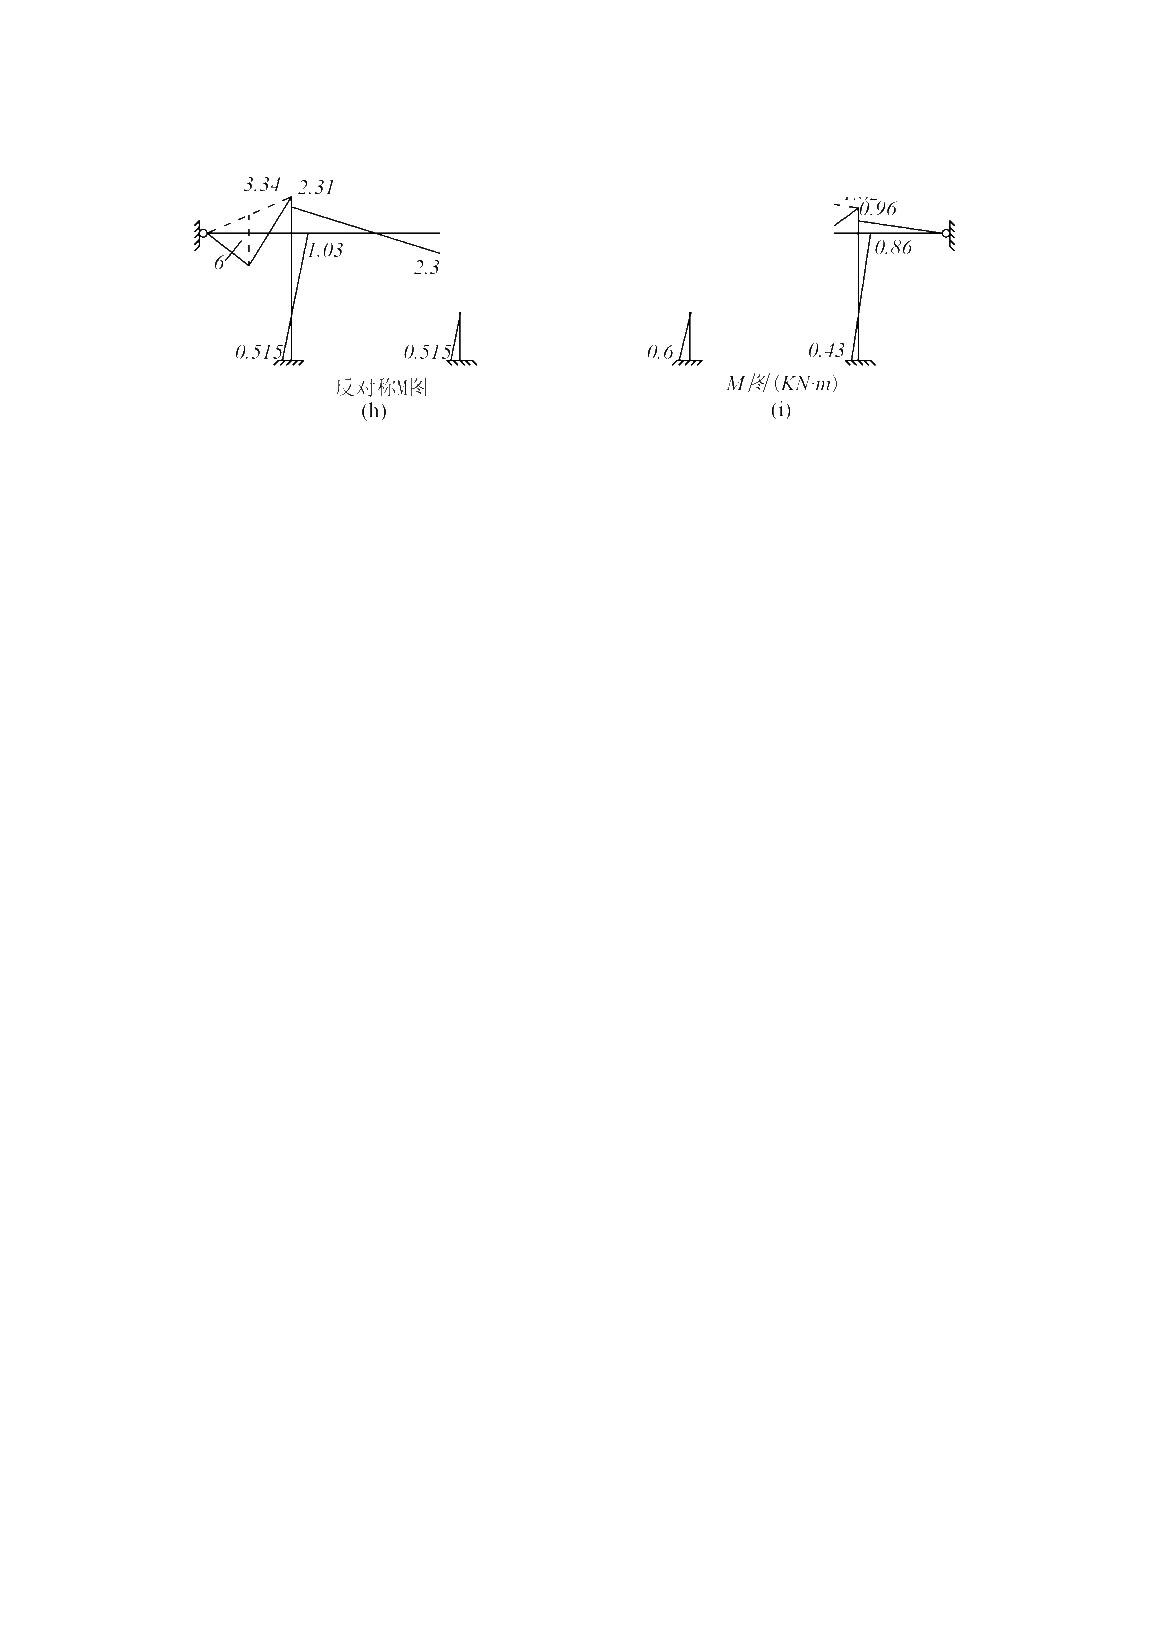
\includegraphics[width=0.92\textwidth]{figures/src15_p020.jpg}
\caption{结构力学基础与技巧班第12次作业及答案（位移法） 第 20 页清理图形页}
\end{figure}
\subsection*{第 21 页转写}
OOOUGUGUG

F12

5Fp/18

5Fpl/18

Fpl/6

Fpl/6

Fp/18

5Fpl/18

2Fp/9

5Fpl/18

Fpl/6

Fp/18

2Fpl/9

2Fpl/9

M图
\begin{figure}[H]\centering
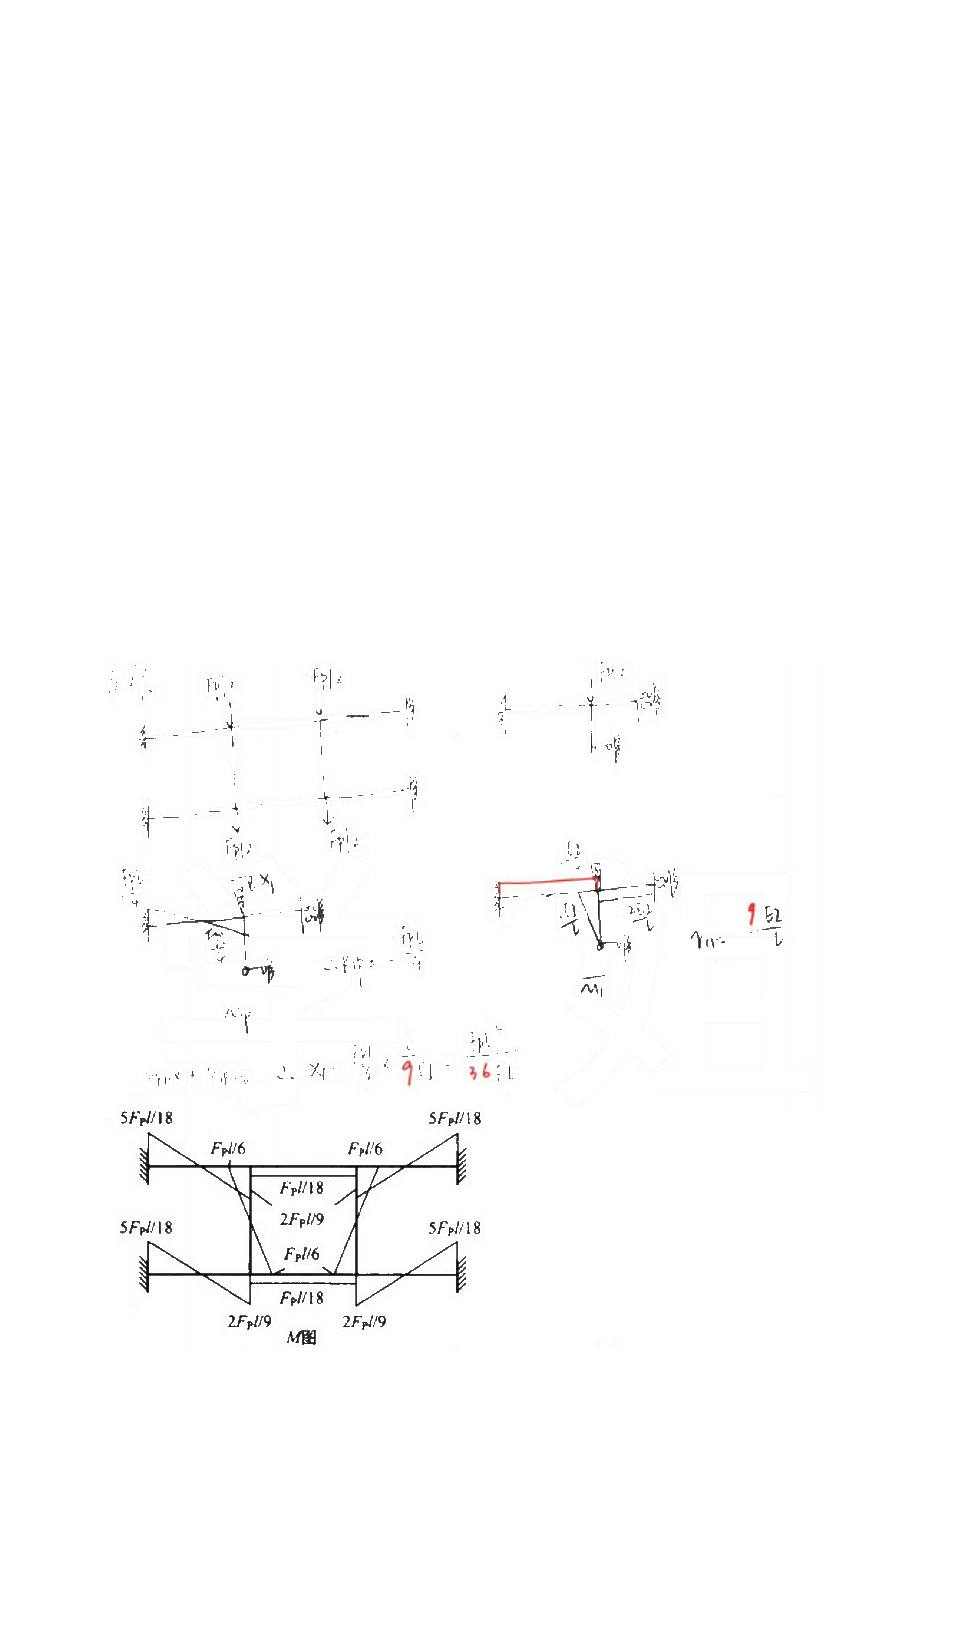
\includegraphics[width=0.92\textwidth]{figures/src15_p021.jpg}
\caption{结构力学基础与技巧班第12次作业及答案（位移法） 第 21 页清理图形页}
\end{figure}
\subsection*{第 22 页转写}
6-8.

(4)

24+
\begin{figure}[H]\centering
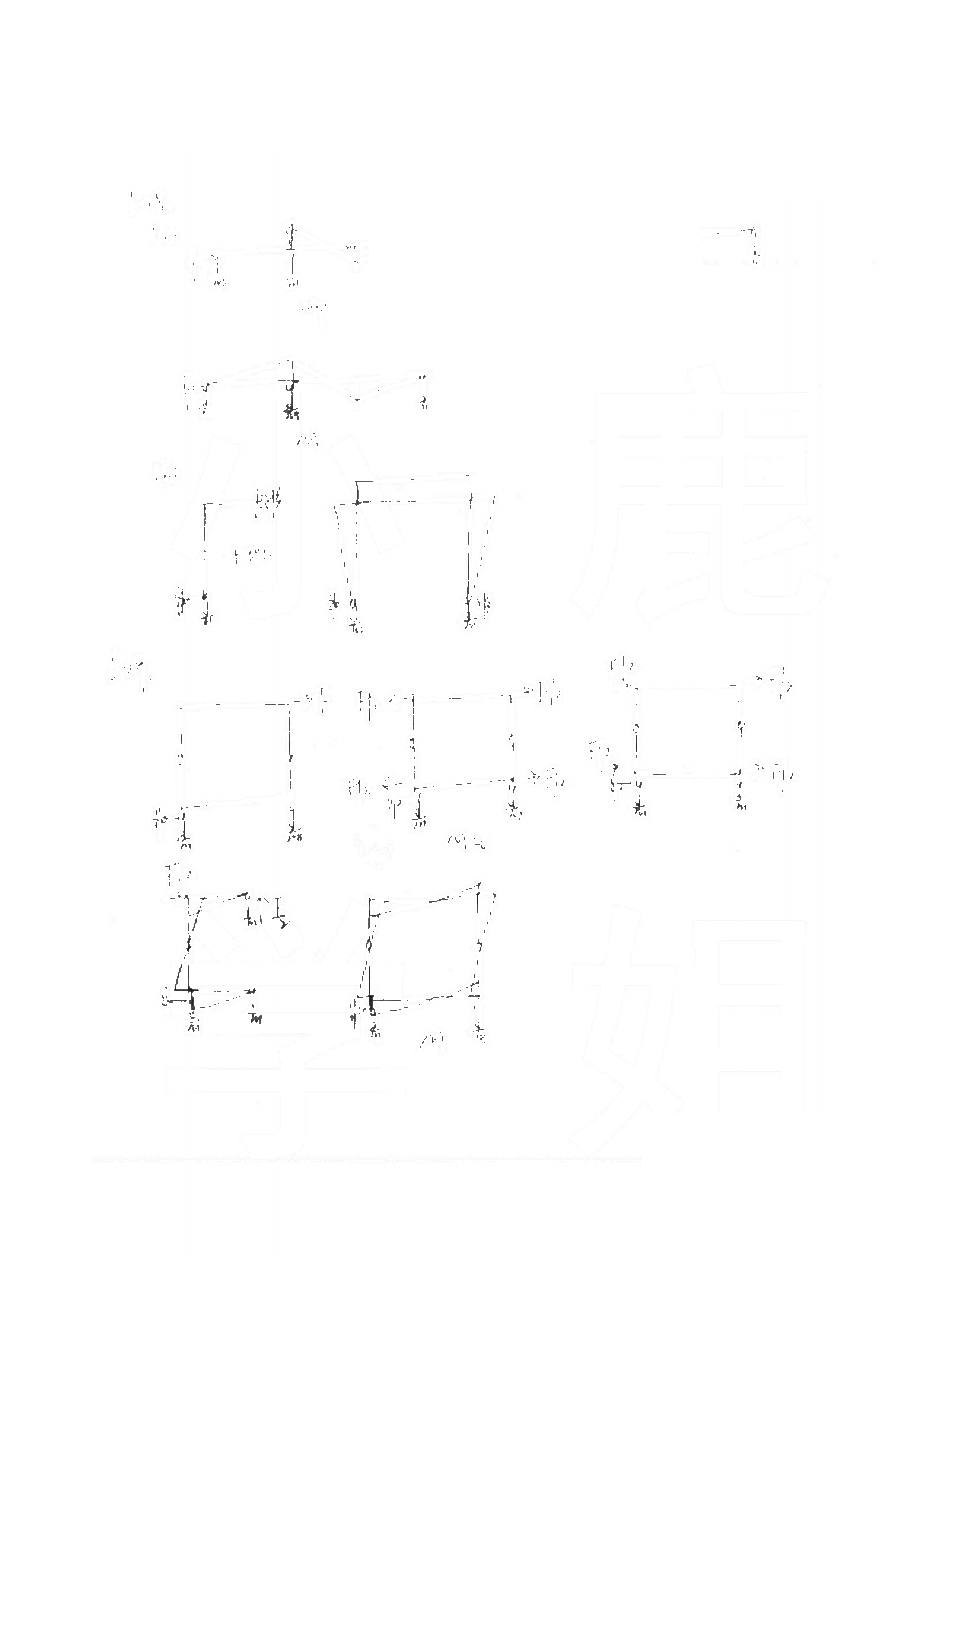
\includegraphics[width=0.92\textwidth]{figures/src15_p022.jpg}
\caption{结构力学基础与技巧班第12次作业及答案（位移法） 第 22 页清理图形页}
\end{figure}
\subsection*{第 23 页转写}
6-30

149

13

191

48o
\begin{figure}[H]\centering
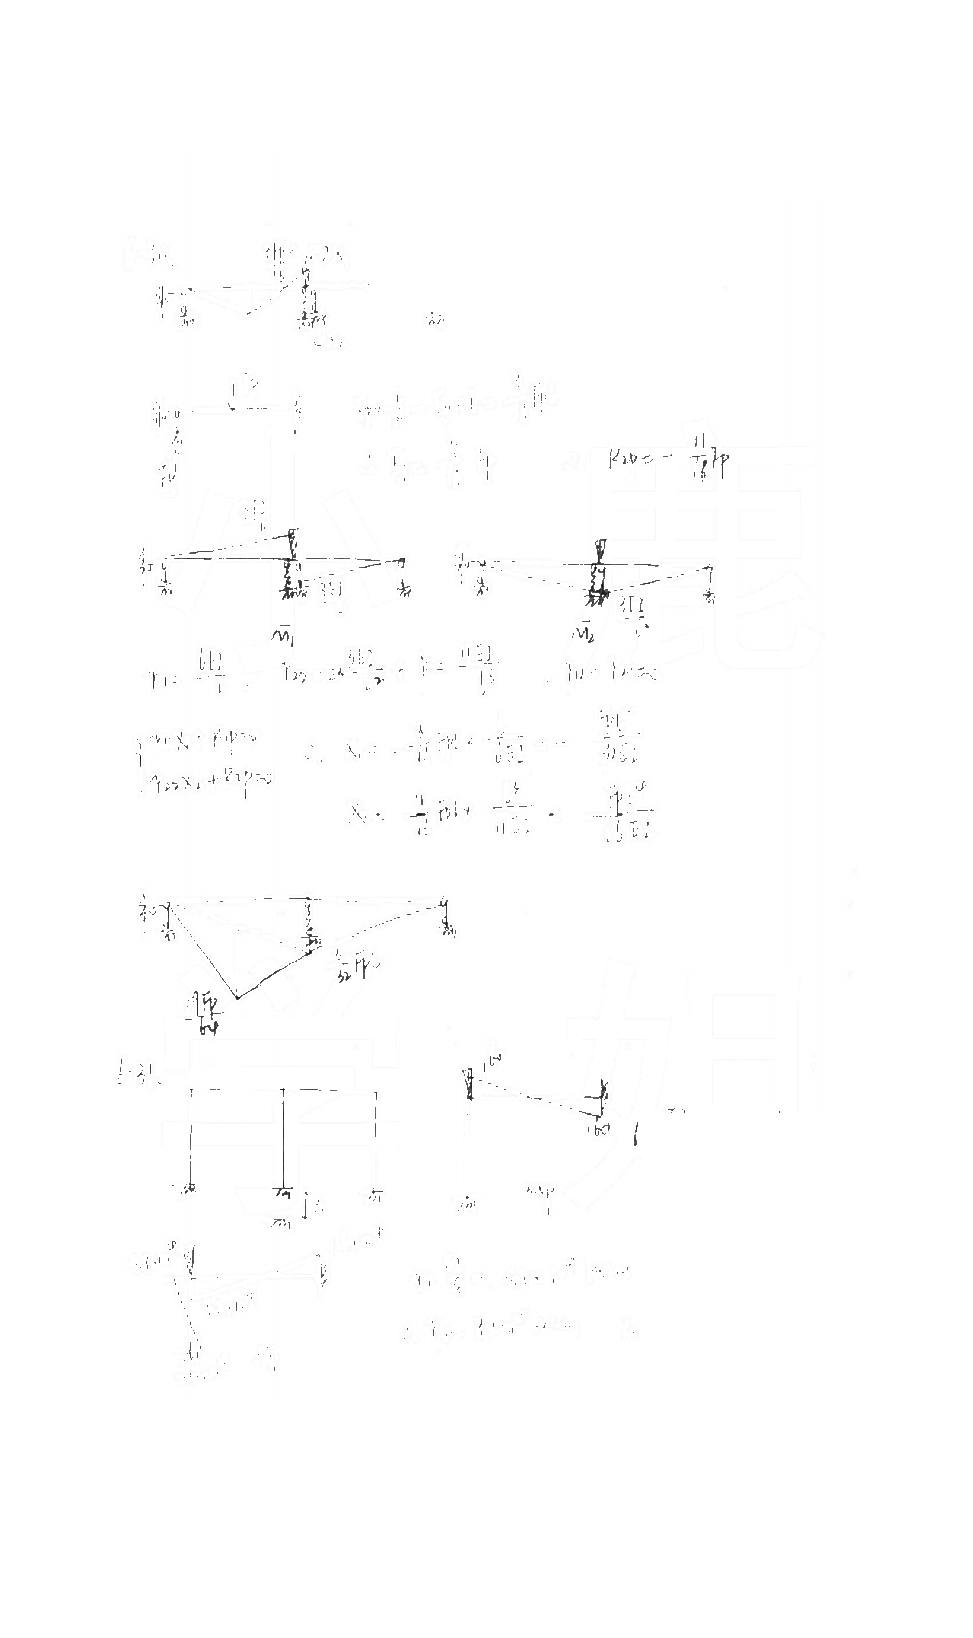
\includegraphics[width=0.92\textwidth]{figures/src15_p023.jpg}
\caption{结构力学基础与技巧班第12次作业及答案（位移法） 第 23 页清理图形页}
\end{figure}
\subsection*{第 24 页转写}
96

96
\begin{figure}[H]\centering
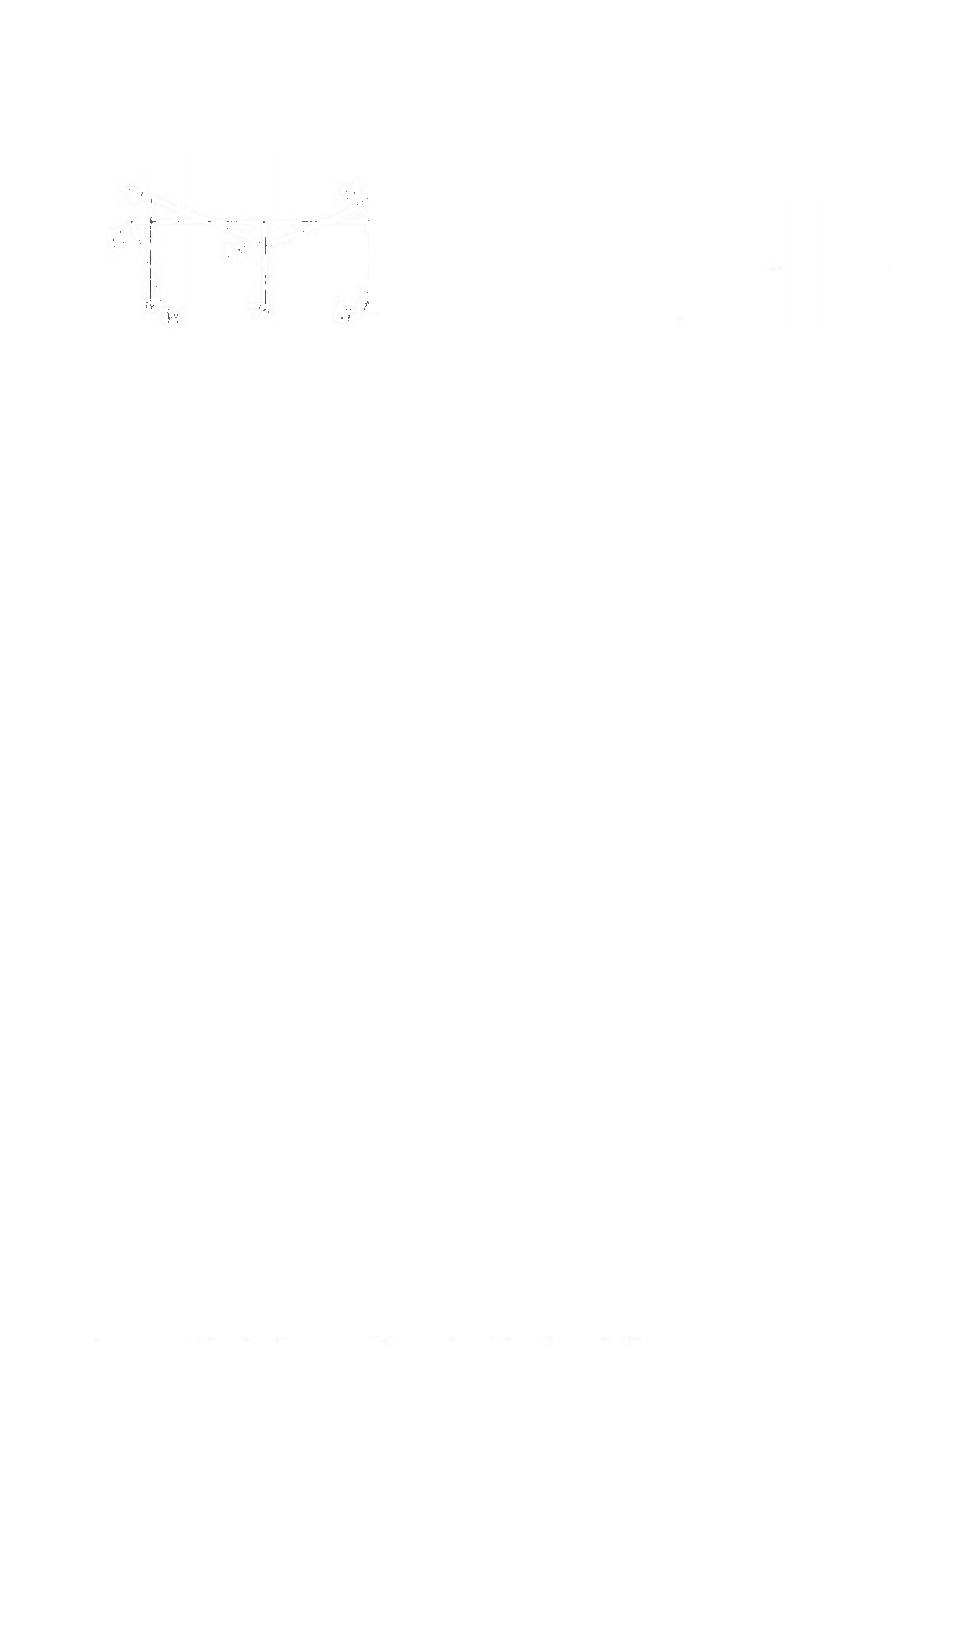
\includegraphics[width=0.92\textwidth]{figures/src15_p024.jpg}
\caption{结构力学基础与技巧班第12次作业及答案（位移法） 第 24 页清理图形页}
\end{figure}
\subsection*{第 25 页转写}
6-32、

解：可将原结构支座位移分解为正对称和反对称两种情况，其中正对称下结构没有内力可不

考虑，取反对称半结构，由于竖杆为剪力静定杆，故水平线位移可不作为位移法基本未知量，

取位移法基本体系见图（a），位移法方程为11

1

1

0

P

r X

R

+

=

。画出

1

M 图和M P 图如图（b）

（c）所示，各系数和自由项为

11

13

r

i

=

，

1

12

P

i

R

l

\textbackslash{}Delta

=  

将系数和自由项代入位移法方程

1

12

13

0

i

iX

l

\textbackslash{}Delta

 

=

，解方程得

1

12

13

X

l

\textbackslash{}Delta

=

。由对称性

M=11 + M叠加得原结构最后弯矩图，如图（d）所示。
\begin{figure}[H]\centering
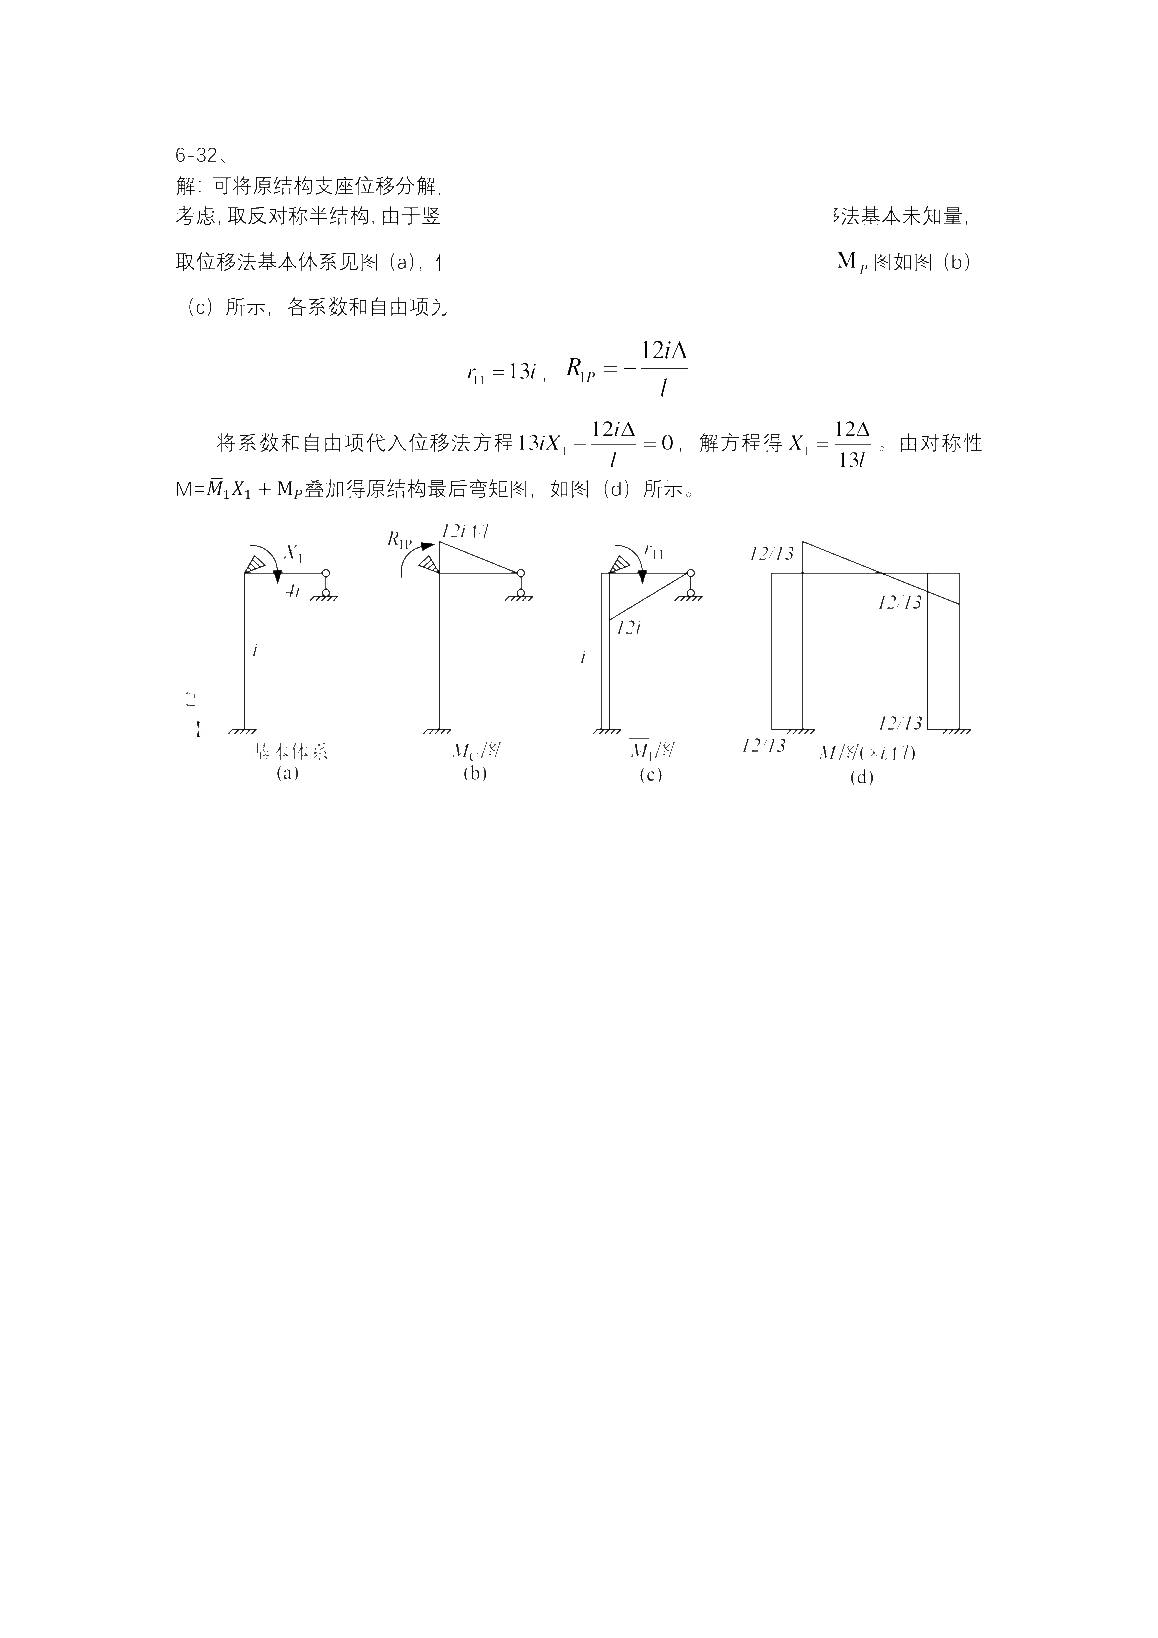
\includegraphics[width=0.92\textwidth]{figures/src15_p025.jpg}
\caption{结构力学基础与技巧班第12次作业及答案（位移法） 第 25 页清理图形页}
\end{figure}
\subsection*{第 26 页转写}
6-32

解：可将支座位移分解为正对称加反对称两种情况，其中正对称下没有弯矩可不

考虑，取反对称半结构，位移法基本体系如图（a）所示。其中竖杆为剪力静定

杆，可不考虑线位移为基本未知量。画出

1

M 图和

C

M 图，如图（b）（c）所示。

位移法方程为11

1

1C

0

r X

R

+

=

。各系数和自由项为：11

13

r

i

=

,

1C

12i

R

l

\textbackslash{}Delta

=

。将系数

和自由项代入位移法方程，得

1

12

13

0

i

iX

l

\textbackslash{}Delta

+

=

，解方程得

1

12

13

X

l

\textbackslash{}Delta

=

。利用叠加公

式M=

1

1

C

M

M X +

，M 图如图（d）所示。

6-33

解：结构有3 个独立位移，加上三个附加约束，画出基本体系[见图(a)]。画出

1

M 、

2

M 、

3

M 图和

P

M 图[见图(b)\textasciitilde{}(e)]，列出位移法方程







=

+

+

+

=

+

+

+

=

+

+

+

0

0

0

3

3

33

2

32

1

31

2

3

23

2

22

1

21

1

3

13

2

12

1

11

P

P

P

R

X

r

X

r

X

r

R

X

r

X

r

X

r

R

X

r

X

r

X

r

计算刚度系数和自由项，即

l

EI

r

8

11 =

，

2

21

12

5

l

EI

r

r

-

=

=

，

2

31

13

6 l

EI

r

r

-

=

=

，

3

22

13 l

EI

r

=

，

0

32

23

=

=r

r

，

3

33

18 l

EI

r

=

8

3

2

1

ql

R P =

，

4

5

2

ql

R P

-

=

，

8

5

3

ql

R P

-

=
\begin{figure}[H]\centering
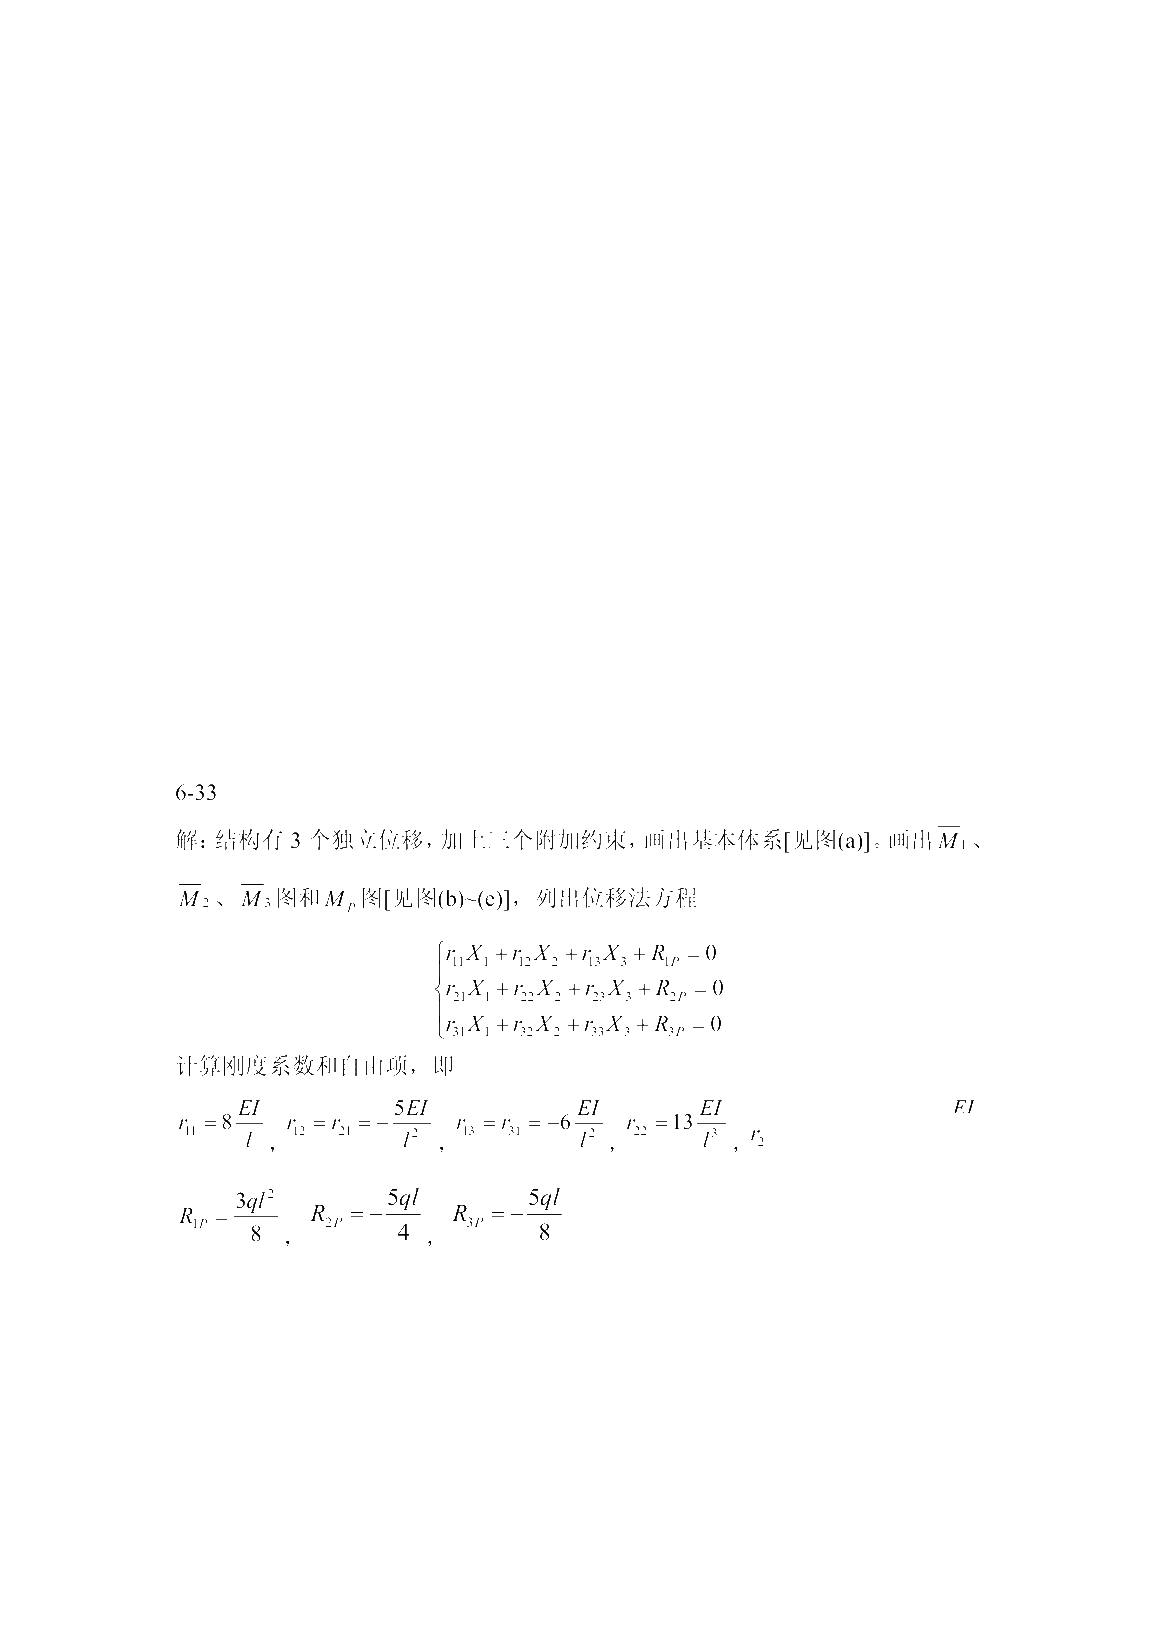
\includegraphics[width=0.92\textwidth]{figures/src15_p026.jpg}
\caption{结构力学基础与技巧班第12次作业及答案（位移法） 第 26 页清理图形页}
\end{figure}
\subsection*{第 27 页转写}
(a) 基本体系

(b)  1图

(c)  2图

(d)  3图

(e)   图

代入位移法方程，即



















=

-

+

-

=

-

+

-

=

+

-

-

0

8

5

18

6

0

4

5

13

5

0

8

3

6

5

8

3

3

1

2

2

3

1

2

2

3

2

2

2

1

ql

X

l

EI

X

l

EI

ql

X

l

EI

X

l

EI

ql

X

l

EI

X

l

EI

X

l

EI

，



















=

=

=

EI

ql

X

EI

ql

X

EI

ql

X

7632

461

159

20

636

49

4

3

4

2

3

1
\begin{figure}[H]\centering
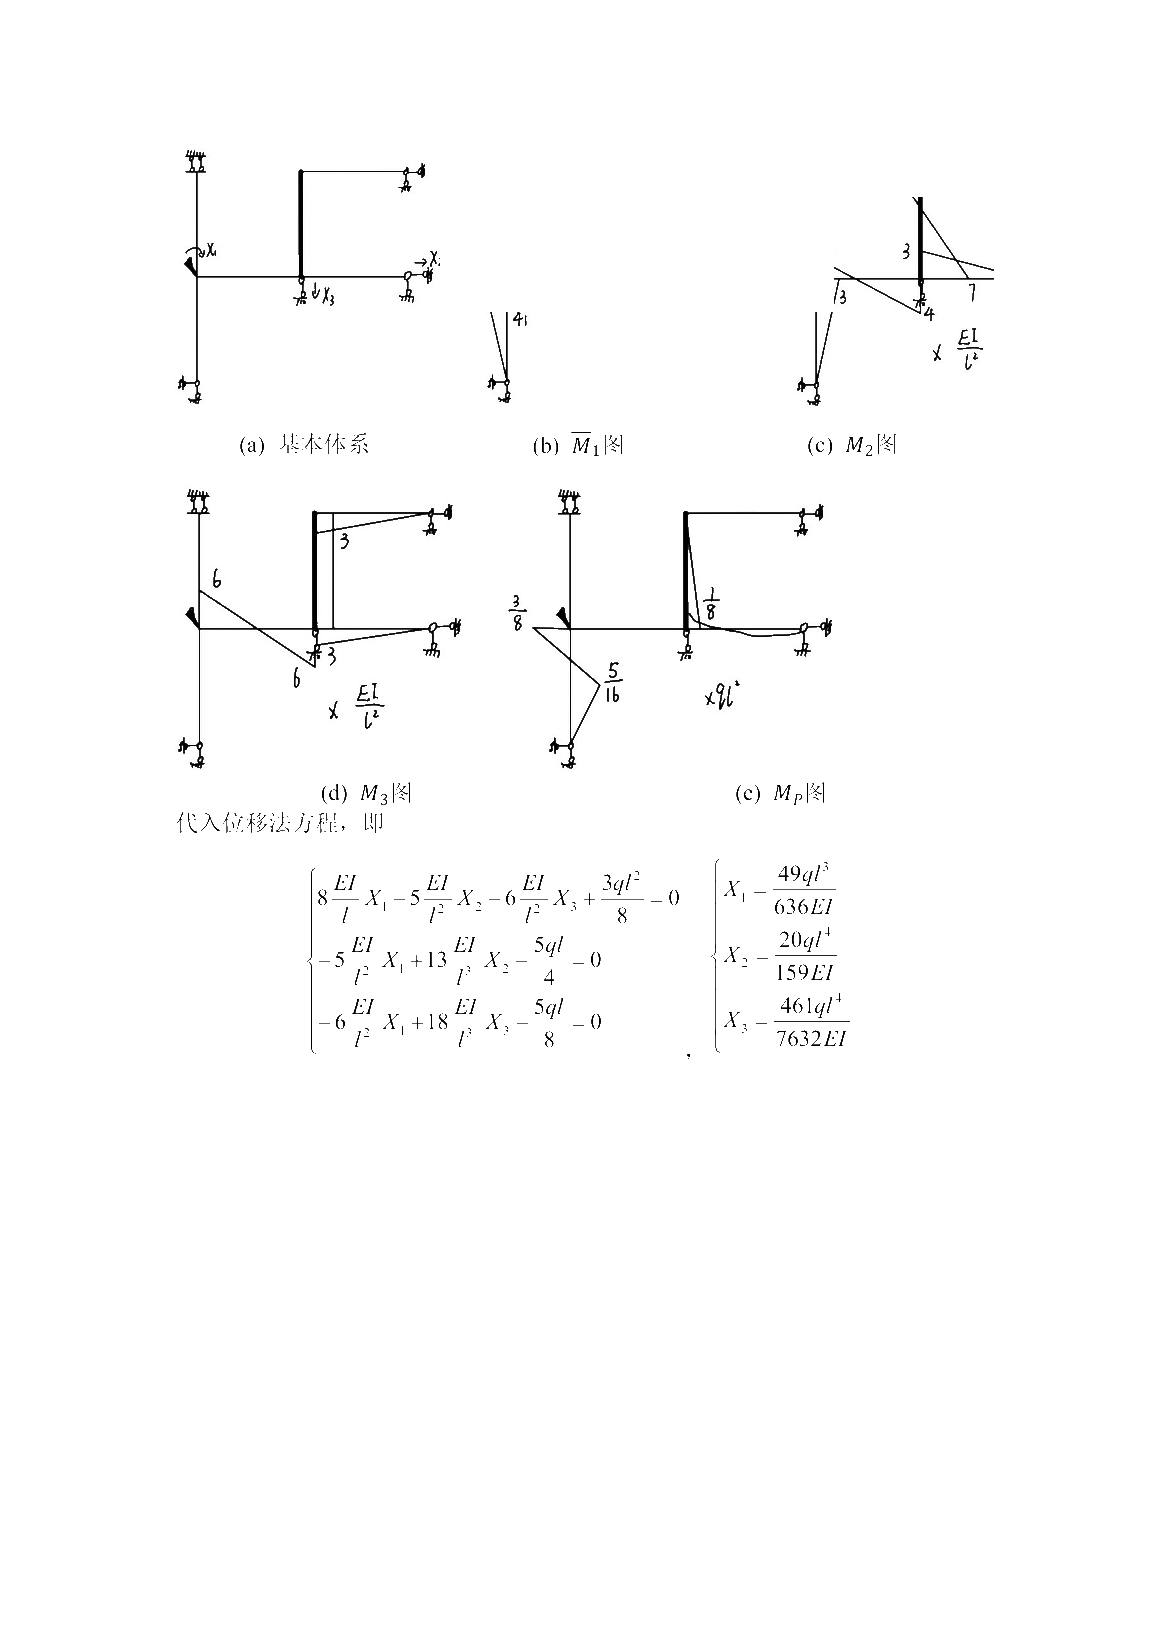
\includegraphics[width=0.92\textwidth]{figures/src15_p027.jpg}
\caption{结构力学基础与技巧班第12次作业及答案（位移法） 第 27 页清理图形页}
\end{figure}
\subsection*{第 28 页转写}
6 -34

6626

TXRP=ocXI=
\begin{figure}[H]\centering
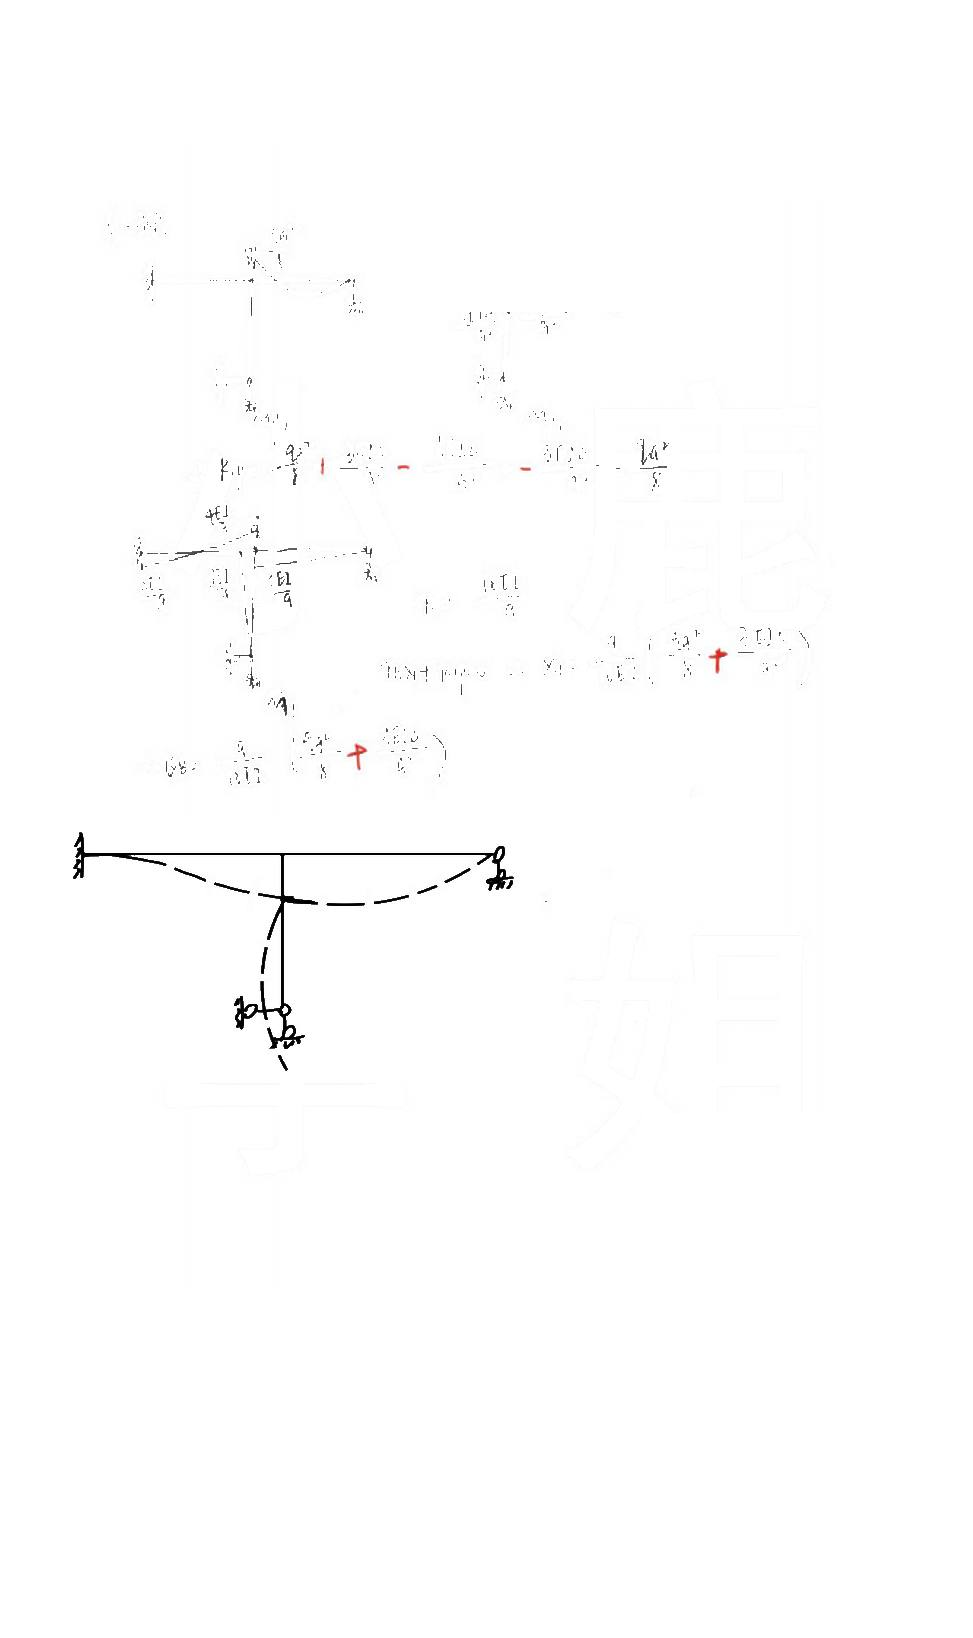
\includegraphics[width=0.92\textwidth]{figures/src15_p028.jpg}
\caption{结构力学基础与技巧班第12次作业及答案（位移法） 第 28 页清理图形页}
\end{figure}
